% Auto-extracted from ../tfpt-42.tex for the TFPT 4.5 clean split.
% Source body assigned by the TFPT 4.5 clean split.

% ---- Kernel numerics and electromagnetic closure: source lines 2315-2695 ----
\section{Kernel numerics and electromagnetic closure}

The boundary-to-carrier presentation should not leave the impression that TFPT is hard only at the level of group theory and representation bookkeeping. The numerical kernel already fixes a nontrivial output layer. Here that layer is pulled forward and read as the first established output package of the carrier/output architecture rather than as a later list of disconnected constants.

\begin{theorem}[Primitive seam generator]
\label{thm:primitive-seam-generator}
The primitive relative seam loop defines the positive generator
\[
[u_\Sigma]=1\in K^1(S^1)\cong \mathbb Z.
\]
Hence the associated seam spectral flow is
\[
SF(U_\Seam)=1,
\qquad
\Delta_\Seam=2\pi.
\]
In the relative Chern normalization, the seam constant is
\[
\cthree:=\frac{\Delta_\Seam}{16\pi^2}=\frac{1}{8\pi}.
\]
Moreover the seam-even base opening is the normalized complement of the carrier quadratic norm,
\[
\phibase
:=
\frac{1-\gamma}{\pi}
=
\frac{1-\tr_EY^2}{\pi}
=
\frac{1}{6\pi}.
\]
\end{theorem}

\begin{proof}[Proof sketch]
The primitive reconstruction yields one elementary relative seam class and therefore one primitive
generator of the seam $K^1$ lattice. Along a single positive seam circuit the spectral flow changes
by one, so the associated loop has class $[u_\Sigma]=1$ and spectral flow $SF(U_\Seam)=1$. The
primitive circuit closes after one full turn, giving $\Delta_\Seam=2\pi$ and hence
$\cthree=\Delta_\Seam/(16\pi^2)=1/(8\pi)$. The carrier theorem gives
$\gamma=\tr_EY^2=5/6$, so the seam-even opening is the normalized complement of the carrier
quadratic norm rather than a new independent numerical input.
\end{proof}

\begin{remark}[Interpretive picture of the primitive start state]
At the level of physical intuition, the primitive spectral seed may be read as a minimal nontrivial relative defect state: two sheets, one seam, one elementary relative winding, and an undecomposed internal rank-$5$ kernel before the carrier split is imposed. This is only an interpretive picture, not a new theorem. Its role is to explain why the earliest hard numbers $(\cthree,\phibase)$ already look like seam-normalized responses of a genuinely relative starting configuration.
\end{remark}

\begin{figure}[t]
\centering
\scriptsize
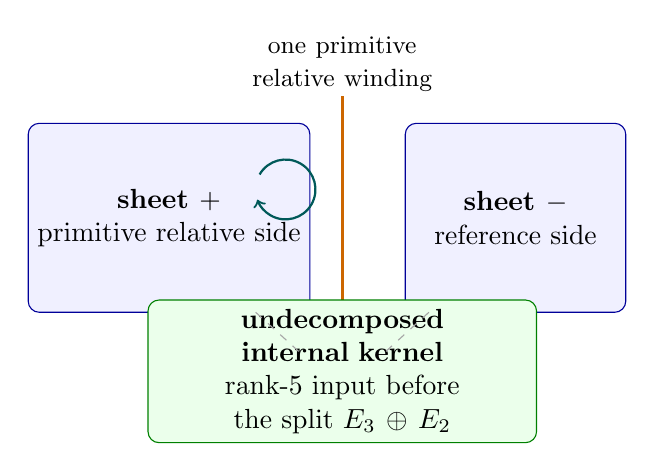
\begin{tikzpicture}[
    sheet/.style={draw=blue!60!black, fill=blue!6, rounded corners, minimum width=2.8cm, minimum height=2.4cm, align=center},
    kernel/.style={draw=green!50!black, fill=green!8, rounded corners, text width=4.7cm, minimum height=0.95cm, align=center}
]
\node[sheet] (up) at (-2.2,0) {\textbf{sheet $+$}\\primitive relative side};
\node[sheet] (down) at (2.2,0) {\textbf{sheet $-$}\\reference side};
\draw[orange!80!black, line width=1.2pt] (0,-1.55) -- (0,1.55);
\node[orange!80!black, above] at (0,1.55) {$\Seam$};
\draw[->, thick, teal!70!black] (-1.05,0.55) arc[start angle=150,end angle=-160,radius=0.38];
\node[align=center, text width=3.0cm] at (0,1.95) {\small one primitive\\relative winding};
\node[kernel] (k) at (0,-1.95) {\textbf{undecomposed internal kernel}\\rank-$5$ input before the split $E_3\oplus E_2$};
\draw[dashed, gray!70] (-1.1,-1.2) -- (-0.55,-1.7);
\draw[dashed, gray!70] (1.1,-1.2) -- (0.55,-1.7);
\end{tikzpicture}
\caption{Interpretive primitive start sketch. Two sheets, one seam, one elementary relative winding,
and an undecomposed rank-$5$ kernel appear before the later split into $E_3\oplus E_2$.
The picture is heuristic only; the theorem-level data are reconstructed from the one-sided
boundary datum.}
\label{fig:primitive-start-sketch}
\end{figure}

\subsection{Carrier form of the electromagnetic closure}

At this stage the electromagnetic closure is kept in generic closed form. The hard carrier data
fix
\[
\cthree=\frac{1}{8\pi},
\qquad
\phibase=\frac{1}{6\pi},
\]
while the later family and Higgs theorems will specialize the abelian index coefficient and the
topological bridge coefficient.

\begin{proposition}[Carrier susceptibility exponent]
\label{prop:carrier-susceptibility-exponent}
On the minimal carrier branch,
\[
B\gamma=\frac32\cdot\frac56=\frac54.
\]
\end{proposition}
\begin{definition}[Minimal primitive seam transfer]
\label{def:exact-seam-generating-function}
Let $\psi_{\Sigma}$ be the normalized primitive seam mode singled out by
\TFPTxref{thm:primitive-seam-generator}. Define the minimal seam transfer operator by the rank-one
projector
\[
U_{\Sigma}^{\min}:=|\psi_{\Sigma}\rangle\langle\psi_{\Sigma}|.
\]
With
\[
q(\alpha):=\deltatop e^{-2\alpha},
\qquad
B\gamma=\frac54,
\]
one has
\[
\mathcal W_{\Sigma}(\alpha)
:=
-B\gamma\,\tr_{\mathrm{adm}}\log\!\bigl(1-q(\alpha)U_{\Sigma}^{\min}\bigr)
=-\frac54\log(1-q(\alpha)).
\]
\[
\mathcal T_{\Sigma}(\alpha)=e^{\mathcal W_{\Sigma}(\alpha)}=(1-q(\alpha))^{-5/4}.
\]
\begin{equation}
\label{eq:phi-opening}
\phiseam(\alpha)=\phibase+q(\alpha)(1-q(\alpha))^{-5/4}.
\end{equation}
\end{definition}

\begin{proposition}[Normalized scalar closure potential]
\label{prop:log-det-variation-u1}
Let
\[
F_{U(1)}(\alpha):=\alpha^3-2\cthree^3\alpha^2-8\cthree^6 b_1\log\bigl(\phiseam(\alpha)^{-1}\bigr).
\]
There exists a unique quartic local counterterm $P_{\mathrm{loc}}$ satisfying
\[
P_{\mathrm{loc}}(0)=P_{\mathrm{loc}}'(0)=0,
\qquad
P_{\mathrm{loc}}'(\alpha)=\alpha^3-2\cthree^3\alpha^2,
\]
namely
\[
P_{\mathrm{loc}}(\alpha)=\frac{\alpha^4}{4}-\frac23\cthree^3\alpha^3.
\]
Hence the normalized scalar closure potential
\[
\Gamma_{U(1)}(\alpha)
:=
\frac{\alpha^4}{4}-\frac23\cthree^3\alpha^3
-8\cthree^6 b_1\int_0^\alpha \log\bigl(\phiseam(a)^{-1}\bigr)\,da
\]
satisfies
\[
\partial_{\alpha}\Gamma_{U(1)}(\alpha)=F_{U(1)}(\alpha).
\]
\end{proposition}


\iffalse
\begin{theorem}[Exact electromagnetic closure on the minimal seam mode]
\label{thm:exact-electromagnetic-closure}
\label{thm:alpha-canonical}
On the canonical branch one has
\[
\cthree=\frac{1}{8\pi},
\phibase=\frac{1}{6\pi},
\qquad
\deltatop=\frac{3}{256\pi^4},
\qquad
b_1=\frac{41}{10}.
=0.
\]
On the admissible interval there is a unique positive solution $\alpha_\star$.
\end{theorem}

\begin{proof}[Proof sketch]
By \Cref{prop:log-det-variation-u1}, the Euler--Lagrange equation for
$\Gamma_{U(1)}$ is exactly the displayed fixed-point equation. Near $\alpha=0$ the logarithmic term
dominates with negative sign, whereas for large $\alpha$ the cubic term dominates positively. By
\Cref{lem:phi-monotone}, the seam contribution varies monotonically on the admissible interval, so
after the tiny carrier-scale start region there is only one admissible sign change. Hence the
closed branch carries one positive fixed point $\alpha_\star$.
\end{proof}

\fi

\begin{theorem}[Exact electromagnetic closure on the minimal seam mode]
\label{thm:exact-electromagnetic-closure}
\label{thm:alpha-canonical}
On the canonical branch one has
\[
\cthree=\frac{1}{8\pi},
\qquad
\phibase=\frac{1}{6\pi},
\qquad
\deltatop=\frac{3}{256\pi^4},
\qquad
\sum_{f,j}L_{f,j}^{\mathrm{diag}}+N_\Phi=40+1=41.
\]
With the rank-one seam transfer of \Cref{def:exact-seam-generating-function}, the closure equation
is the scalar equation
\begin{equation}
\label{eq:carrier-cfe}
F_{U(1)}(\alpha)=0,
\qquad
F_{U(1)}(\alpha)=\alpha^3-2\cthree^3\alpha^2-\frac45\cthree^6
\left(\sum_{f,j}L_{f,j}^{\mathrm{diag}}+N_\Phi\right)\log\bigl(\phiseam(\alpha)^{-1}\bigr),
\end{equation}
where
\[
\phiseam(\alpha)=\frac{1}{6\pi}+\frac{3e^{-2\alpha}}{256\pi^4}
\left(1-\frac{3e^{-2\alpha}}{256\pi^4}\right)^{-5/4}.
\]
This equation has a unique positive root
\[
\alpha_{\star}=0.00729735256220985312786969108226575414\dots
\]
and therefore
\[
\alpha_{\star}^{-1}=137.03599921684071250353786030380388037\dots.
\]
\end{theorem}

\begin{proof}
The explicit formulas above follow from the rank-one determinant identity
\[
\det(1-qU_{\Sigma}^{\min})=1-q
\qquad
\text{for } U_{\Sigma}^{\min}=|\psi_{\Sigma}\rangle\langle\psi_{\Sigma}|.
\]
The derivative of the closure function is
\[
F_{U(1)}'(\alpha)
:=
3\alpha^2-4\cthree^3\alpha
-\frac85\cthree^6\left(\sum_{f,j}L_{f,j}^{\mathrm{diag}}+N_\Phi\right)\,
\frac{q(\alpha)(1-q(\alpha))^{-9/4}\bigl(1+q(\alpha)/4\bigr)}
{\phibase+q(\alpha)(1-q(\alpha))^{-5/4}}.
\]
On $[0,2\cdot 10^{-4}]$ one verifies by interval arithmetic that
\[
F_{U(1)}(\alpha)<0.
\]
On $[2\cdot 10^{-4},10^{-1}]$ one verifies by interval arithmetic that
\[
F_{U(1)}'(\alpha)>0.
\]
Finally
\[
F_{U(1)}(10^{-2})>0.
\]
Therefore $F_{U(1)}$ crosses zero exactly once. The displayed numerical root is obtained by
monotone bisection on that interval.
\end{proof}

\begin{remark}[Asymptotic opening as a secondary expansion]
Using \Cref{prop:carrier-susceptibility-exponent}, the determinant output admits the small
opening expansion
\[
\phiseam(\alpha)
=
\phibase
+\deltatop e^{-2\alpha}
+\frac54\deltatop^2e^{-4\alpha}
+O(e^{-6\alpha}),
\]
which should be read only as a secondary expansion of the determinant output, not as the primary
definition of the electromagnetic closure.
\end{remark}

The dependency structure of the electromagnetic closure is displayed in
\Cref{fig:alpha-closure-flow}. What matters is not one formula in isolation, but the fact that
the same carrier-side inputs fix the rank-one determinant, the scalar closure potential, and the
fixed-point equation in one direction. The later transport and Higgs theorems then specialize the
budget $\sum_{f,j}L_{f,j}^{\mathrm{diag}}+N_\Phi$ and $\deltatop$ to their canonical closed values.
\begin{remark}[Logarithmic scale closure of the electromagnetic equation]
Define the internally generated logarithmic scale
\[
\mu_\Sigma(\alpha):=(\phiseam(\alpha))^{-1}.
\]
Then \TFPTxref{eq:carrier-cfe} is equivalent to
\[
\ln \mu_\Sigma(\alpha)
=
\frac{\alpha^2\bigl(\alpha-2\cthree^3\bigr)}
{\frac45\cthree^6\left(\sum_{f,j}L_{f,j}^{\mathrm{diag}}+N_\Phi\right)}.
\]
Thus the observed fine-structure constant is selected by a balance between a geometric cubic term
and a self-generated logarithmic scale parameter. This is RG-like and transmutation-like,
because the coefficient is the internally closed transport-plus-Higgs budget divided by $10$, and
the logarithm is attached to an internally produced scale. In the present paper it should be read
as \emph{logarithmic scale closure} or a geometric fixed-point equation rather than as an externally
prescribed one-loop running law. The symbol $\mu_\Sigma(\alpha)$ here is local to the
electromagnetic closure discussion and should not be confused with the later matching scale
$M_\Sigma$.
\end{remark}
A related appendix continuation records that with
\[
g:=5,
\qquad
d:=\dim \mathfrak g_{\SM}=12,
\]
\[
\gcd(\Oadm,\Dstart)=d,
\qquad
\operatorname{lcm}(\Oadm,\Dstart)=g(g-1)d=240=|R(E_8)|.
\]

\begin{figure}[t]
\centering
\scriptsize
\begin{tikzpicture}[
    >=Latex,
    node distance=8mm and 10mm,
    hard/.style={draw=blue!60!black, fill=blue!6, rounded corners, align=center, text width=2.2cm, minimum height=0.9cm},
    closure/.style={draw=orange!75!black, fill=orange!8, rounded corners, align=center, text width=2.8cm, minimum height=0.95cm},
    outbox/.style={draw=green!50!black, fill=green!8, rounded corners, align=center, text width=3.0cm, minimum height=0.95cm}
]
\node[hard] (c3) {$\cthree=\dfrac{1}{8\pi}$};
\node[hard, right=of c3] (bg) {$B\gamma=\dfrac54$};
\node[hard, right=of bg, text width=2.7cm] (budget) {$\sum L_{f,j}^{\mathrm{diag}}+N_\Phi=41$};

\node[closure, below=of bg] (det) {rank-one determinant\\$\mathcal T_\Sigma(\alpha)=(1-\deltatop e^{-2\alpha})^{-5/4}$};
\node[closure, below left=of det] (phi) {determinant output\\$\phiseam(\alpha)=\phibase+\deltatop e^{-2\alpha}(1-\deltatop e^{-2\alpha})^{-5/4}$};
\node[closure, below right=of det] (logdet) {scalar closure potential\\$\partial_\alpha\Gamma_{U(1)}(\alpha)=F_{U(1)}(\alpha)$};
\node[outbox, below=of $(phi)!0.5!(logdet)$, yshift=-2mm, text width=4.6cm] (cfe) {fixed-point equation\\$\alpha^3-2\cthree^3\alpha^2-\frac45\cthree^6\bigl(\sum L_{f,j}^{\mathrm{diag}}+N_\Phi\bigr)\ln((\phiseam(\alpha))^{-1})=0$};
\node[outbox, below=of cfe] (root) {fine-structure fixed point\\interval-rigid on the closed branch};

\draw[->, thick] (c3) -- (det);
\draw[->, thick] (bg) -- (det);
\draw[->, thick] (det) -- (phi);
\draw[->, thick] (det) -- (logdet);
\draw[->, thick] (budget) |- (cfe);
\draw[->, thick] (phi) -- (cfe);
\draw[->, thick] (logdet) -- (cfe);
\draw[->, thick] (cfe) -- (root);
\end{tikzpicture}
\caption{$\alpha$ closure flow in closed form. The carrier data determine the rank-one determinant,
the scalar closure potential, and the fixed-point equation. The numerical specialization is made
only after the transport and Higgs theorems close the branch budget.}
\label{fig:alpha-closure-flow}
\end{figure}

\subsection{Kernel output package}

The benchmark row for $\alpha^{-1}(0)$ is defined by the positive self-consistent root of \TFPTxref{eq:carrier-cfe}, not by freezing the opening at its retained seed value. On the canonical branch that positive root remains
\[
\alpha^{-1}(0)=\num{137.03599921684071}.
\]
For the remaining one-seed relations we keep the retained branch opening
\begin{equation}
\label{eq:hard-kernel-values}
\cthree=\frac{1}{8\pi},
\qquad
\phiz=\frac{1}{6\pi}+\frac{3}{256\pi^4},
\end{equation}
\begin{remark}[Exact opening versus retained seed]
The two symbols belong to the same admissible branch but play different jobs. The electromagnetic $\alpha$ row uses the exact seam generating function $\phiseam(\alpha)$ inside the carrier-form closure equation, whereas the one-seed bridge relations freeze that branch to the retained canonical seed $\phiz$. Thus $\phiseam(\alpha)$ belongs only to the exact $\alpha$ benchmark line, while $\phiz$ is the seed used for $(\beta_{\mathrm{rad}},\Omega_b,\lambda_C,\sin^2\theta_{13})$.
\end{remark}
and the same retained kernel package emits the compact seed chain
\begin{equation}
\label{eq:kernel-benchmark-formulas}
\begin{aligned}
C_{a\gamma\gamma}&=-4\cthree=-\frac{1}{2\pi},
&
\beta_{\mathrm{rad}}&=\frac{\phiz}{4\pi},
\\
\Omega_b&=(4\pi-1)\beta_{\mathrm{rad}},
&
\lambda_C&=\sqrt{\phiz(1-\phiz)},
\\
\sin^2\theta_{13}&=\phiz e^{-\gamma}.
\end{aligned}
\end{equation}
\begin{remark}[Why the $\alpha$ row must stay self-consistent]
The exact self-consistent equation with $\phiseam(\alpha)$ yields the benchmark value
\[
\alpha^{-1}(0)=\num{137.03599921684071}.
\]
Its second-order truncation reproduces the first two correction coefficients, but it is not itself the benchmark definition. If one instead freezes the opening at
\[
\phiz=\frac{1}{6\pi}+\frac{3}{256\pi^4},
\]
the root shifts to $\alpha^{-1}(0)\approx \num{137.036501465}$, i.e. by about $\num{5.02e-4}$, which is roughly $\num{2.4e4}\sigma$ on the CODATA/NIST uncertainty. The wording of the $\alpha$ benchmark must therefore remain explicit: the benchmark uses the exact seam generating function, while the quadratic formula is only its controlled asymptotic shadow.
\end{remark}
\begin{tcolorbox}[colback=tfptblue!3, colframe=tfptblue, breakable,
    title={Kernel-output package}, colbacktitle=tfptblue]
The point of this section is not to claim more numerics than TFPT currently owns. It is to show that the established kernel already fixes a coherent electromagnetic package before the later completion theorems begin: the seam constant $\cthree$, the retained canonical seed $\phiz$, the self-consistent carrier-form CFE for $\alpha$, the dimensionless axion--photon anomaly coefficient, the birefringence seed, and the Cabibbo anchor.
\end{tcolorbox}


% ---- UV seed shadow, Cabibbo inversion, and alternatives: source lines 3157-3482 ----
\subsection{UV seed-shadow identities and the Cabibbo inversion}

The retained scalar seed $\phiz$ still satisfies exact UV identities. In the present version these
identities are auxiliary kernel bookkeeping rather than the independence grammar of the physical
observable layer. In particular, the Cabibbo angle admits an explicit inversion back to the UV
seed:
\begin{equation}
\label{eq:cabibbo-inversion}
\phiz=\frac{1-\sqrt{1-4\lambda_C^2}}{2}.
\end{equation}
\begin{remark}[Catalan expansion of the Cabibbo inversion]
Setting
\[
x:=\lambda_C^2,
\]
the inversion formula becomes
\[
\phiz=x\,C(x),
\qquad
C(x):=\frac{1-\sqrt{1-4x}}{2x}.
\]
Hence
\begin{equation}
\label{eq:catalan-cabibbo}
\phiz
=
\sum_{n\ge 0} C_n\,\lambda_C^{2n+2}
=
\lambda_C^2+\lambda_C^4+2\lambda_C^6+5\lambda_C^8+14\lambda_C^{10}+\cdots,
\end{equation}
where $C_n$ are the Catalan numbers. In the present paper the appropriate interpretation of this
identity is noncrossing combinatorics on the seed side; it is a theorem-level strengthening of
the one-seed compression rather than a claim about planar Feynman graphs, a specific large-$N$ /
't Hooft resummation, or a holographic flavor limit.
\end{remark}

\begin{proposition}[Retained seed as one decoder]
\label{prop:retained-seed-decoder}
Set
\[
u:=\phiz.
\]
On the retained branch one has
\[
\lambda_C^2=u(1-u),
\qquad
\beta_{\mathrm{rad}}=\frac{u}{4\pi},
\qquad
\Omega_b=\left(1-\frac{1}{4\pi}\right)u,
\qquad
\sin^2\theta_{13}=e^{-\gamma}u.
\]
Equivalently,
\[
u
=
\frac{1-\sqrt{1-4\lambda_C^2}}{2}
=
4\pi\beta_{\mathrm{rad}}
=
\frac{\Omega_b}{1-\frac{1}{4\pi}}
=
e^\gamma\sin^2\theta_{13}.
\]
Thus the retained branch carries a single decoder
\[
u\longmapsto (\lambda_C,\beta_{\mathrm{rad}},\Omega_b,\theta_{13}).
\]
\end{proposition}

\begin{proof}
The forward identities are exactly the retained-seed bridge relations. The inverse identities follow
from the Cabibbo inversion \TFPTeqref{eq:cabibbo-inversion} and direct elimination of $u$ from the same
four formulas.
\end{proof}

Eliminating the retained seed through the Cabibbo inversion gives the equivalent
$\lambda_C$-only formulas:
\begin{equation}
\label{eq:lambda-c-master}
\begin{aligned}
\beta_{\mathrm{rad}}&=\frac{1-\sqrt{1-4\lambda_C^2}}{8\pi},\\
\Omega_b&=\frac{4\pi-1}{8\pi}\bigl(1-\sqrt{1-4\lambda_C^2}\bigr),\\
\sin^2\theta_{13}&=\frac{e^{-\gamma}}{2}\bigl(1-\sqrt{1-4\lambda_C^2}\bigr).
\end{aligned}
\end{equation}

\begin{corollary}[Vacuum half-circle and UV-angle parametrization]
\label{cor:uv-half-circle}
On the retained UV seed split one has the exact identity
\[
\lambda_C^2+\left(\phiz-\frac12\right)^2=\frac14.
\]
Defining
\[
\sin^2\theta_{\mathrm{UV}}:=\phiz,
\]
one obtains
\[
\lambda_C=\frac12\sin(2\theta_{\mathrm{UV}}),
\qquad
\sin^2\theta_{13}=e^{-\gamma}\sin^2\theta_{\mathrm{UV}},
\qquad
\Omega_b=\left(1-\frac{1}{4\pi}\right)\sin^2\theta_{\mathrm{UV}}.
\]
\end{corollary}

\begin{proof}
The exact seed relation $\lambda_C^2=\phiz(1-\phiz)$ is equivalent to the displayed half-circle
identity after completing the square. The $\theta_{\mathrm{UV}}$ parametrization then follows
immediately from $\sin^2\theta_{\mathrm{UV}}=\phiz$ together with the exact retained-seed formulas
for $\sin^2\theta_{13}$ and $\Omega_b$.
\end{proof}

\begin{corollary}[CKM--PMNS bridge law]
\label{cor:ckm-pmns-bridge-law}
On the closed branch one has the exact relation
\[
\sin^2\theta_{13}
=
\frac{e^{-5/6}}{2}\Bigl(1-\sqrt{1-4\lambda_C^2}\Bigr).
\]
Equivalently,
\[
\lambda_C^2=e^{5/6}\sin^2\theta_{13}-e^{10/6}\sin^4\theta_{13}.
\]
In internal branch form,
\[
\sin^2\theta_{13}=0.0231084351588811\ldots
\]
with no additional fit parameter.
\end{corollary}

\begin{proof}
By \TFPTxref{eq:cabibbo-inversion},
\[
\phiz=\frac{1-\sqrt{1-4\lambda_C^2}}{2}.
\]
By the exact seed identity,
\[
\sin^2\theta_{13}=\phiz e^{-\gamma},
\qquad
\gamma=\frac56.
\]
Substituting $\phiz$ gives the displayed formula.
\end{proof}

\begin{corollary}[Baryon--reactor bridge law]
\label{cor:baryon-reactor-bridge-law}
On the closed branch one has the exact cross-sector relation
\[
\Omega_b
=
\left(1-\frac{1}{4\pi}\right)e^{5/6}\sin^2\theta_{13}
=
\frac{4\pi-1}{8\pi}\Bigl(1-\sqrt{1-4\lambda_C^2}\Bigr).
\]
In internal branch form,
\[
\Omega_b=0.0489406626654501\ldots
\]
with no additional fit parameter.
\end{corollary}

\begin{proof}
The exact seed-budget identities give
\[
\Omega_b=(4\pi-1)\beta_{\mathrm{rad}},
\qquad
\beta_{\mathrm{rad}}=\frac{\phiz}{4\pi},
\qquad
\sin^2\theta_{13}=\phiz e^{-5/6}.
\]
Eliminating $\phiz$ yields the displayed cross-sector identity. Eliminating $\phiz$ instead through
\TFPTxref{eq:cabibbo-inversion} gives the equivalent $\lambda_C$ form.
\end{proof}

\begin{corollary}[Matter-radiation quotient on the retained seed split]
\label{cor:matter-radiation-quotient}
On the retained seed split one has the exact quotient identity
\[
\frac{\Omega_b}{\beta_{\mathrm{rad}}}=4\pi-1.
\]
\end{corollary}

\begin{proof}
This is the direct quotient of the exact retained-seed identities
\[
\Omega_b=(4\pi-1)\beta_{\mathrm{rad}},
\qquad
\beta_{\mathrm{rad}}=\frac{\phiz}{4\pi}.
\]
\end{proof}

\begin{remark}[Interpretive reading of the retained seed split]
The same one-seed decoder carries the exact budget identity
\begin{equation}
\label{eq:seed-budget-identity}
\Omega_b+\beta_{\mathrm{rad}}=\phiz.
\end{equation}
Indeed,
\[
\Omega_b+\beta_{\mathrm{rad}}
=(4\pi-1)\beta_{\mathrm{rad}}+\beta_{\mathrm{rad}}
=4\pi\,\beta_{\mathrm{rad}}
=\phiz.
\]
Both \TFPTxref{cor:matter-radiation-quotient,eq:seed-budget-identity} are exact retained-seed
identities. Any solid-angle or spherical-surface interpretation remains interpretive and is not
used as theorem input.
\end{remark}

Thus on the canonical branch, $\beta$, $\Omega_b$, $\lambda_C$, and $\theta_{13}$ are four exact
projections of the same retained decoder $u=\phiz$. Conversely, $\theta_{13}$ fixes $\lambda_C$ and
$\Omega_b$ through $\phiz=e^\gamma\sin^2\theta_{13}$. This is the derived-consequence layer of the
retained seed split, not a separate independent theorem surface.

\subsection{Carrier comparison of alternative discrete worlds}

The strongest numerical pressure test on the carrier packet is not a further precision hit. It is
that nearby wrong discrete worlds miss the electromagnetic closure decisively.

\begin{proposition}[Numerical comparison of alternative discrete worlds]
\label{thm:carrier-exclusion}
Let
\[
\alpha^{-1}(0;N_{\mathrm{fam}},N_\Phi,\nu^c)
\]
denote the positive self-consistent root of the carrier-form electromagnetic closure equation
\TFPTeqref{eq:carrier-cfe} for the indicated discrete data. Then:
\begin{center}
\small
\sisetup{round-mode=none, group-minimum-digits=20}
\setlength{\tabcolsep}{2pt}
\renewcommand{\arraystretch}{0.96}
\begin{tabularx}{0.98\linewidth}{@{}>{\raggedright\arraybackslash}p{0.21\linewidth}>{\raggedright\arraybackslash}p{0.19\linewidth}>{\raggedleft\arraybackslash}p{0.14\linewidth}>{\raggedleft\arraybackslash}p{0.14\linewidth}Y@{}}
\toprule
Discrete world & Change from canonical & $\alpha^{-1}(0)$ & Residual vs CODATA & Reading \\
\midrule
\textbf{canonical $(3,1,\text{yes})$} & --- & $\mathbf{\num{137.0359992}}$ & $+\num{3.9e-8}$ & \makecell[l]{inside CODATA window\\($+1.87\sigma$)} \\
$N_{\mathrm{fam}}=2$ & one family fewer & $\num{156.094}$ & $+19.1$ & catastrophically excluded \\
$N_{\mathrm{fam}}=4$ & one family more & $\num{124.835}$ & $-12.2$ & catastrophically excluded \\
$N_\Phi=2$ & two light Higgs doublets & $\num{135.946}$ & $-1.09$ & catastrophically excluded \\
no $\nu^c$ & remove right-handed neutrino & $\num{137.0338}$ & $-\num{2.16e-3}$ & \makecell[l]{excluded\\(${\sim}\num{1.03e5}\sigma$)} \\
\bottomrule
\end{tabularx}
\end{center}
\end{proposition}

\begin{proof}[Proof sketch]
Hold fixed
\[
\cthree=\frac{1}{8\pi},
\qquad
\phibase=\frac{1}{6\pi},
\qquad
\gamma=\frac56,
\qquad
B=\frac32,
\]
and solve the positive self-consistent root of the same scalar closure equation on each discrete world:
\[
\alpha^3-2\cthree^3\alpha^2-8\cthree^6\,\bone(N_{\mathrm{fam}},N_\Phi)\ln\!\bigl(\phiseam(\alpha)^{-1}\bigr)=0,
\]
with
\[
\phiseam(\alpha)=\phibase+\deltatop e^{-2\alpha}(1-\deltatop e^{-2\alpha})^{-5/4},
\qquad
\deltatop=\Oadm\cthree^4,
\qquad
\delta_2=\frac54\,\deltatop^2,
\]
and
\[
\bone(N_{\mathrm{fam}},N_\Phi)=\frac43N_{\mathrm{fam}}+\frac1{10}N_\Phi.
\]
For the no-$\nu^c$ row, $\bone$ stays unchanged because $Y(\nu^c)=0$, while the occupancy changes from $\Oadm=48$ to $\Oadm=45$ because the one-family packet drops from $16$ to $15$ states. The same positive-branch solver and tolerance are used for every row, so the deviations are arithmetic consequences of changed discrete data rather than fits.
\end{proof}

\begin{remark}
Two families shift $\alpha^{-1}$ by $+19$, four families by $-12$, and two Higgs doublets by
$-1.09$. Even the mildest alternative---removing $\nu^c$---shifts the value by
$\num{2.16e-3}$, which is $\sim\num{1.03e5}$ times the CODATA uncertainty. This is therefore a
useful comparison pressure test on the canonical branch rather than an additional theorem in the
reconstruction chain.
\end{remark}

\begin{figure}[t]
\centering
\scriptsize
\begin{tikzpicture}[
    >=Latex,
    head/.style={draw=black!65, fill=gray!15, rounded corners, minimum height=0.8cm, align=center, font=\bfseries},
    ok/.style={draw=green!50!black, fill=green!8, rounded corners, minimum height=0.8cm, align=left},
    bad/.style={draw=red!70!black, fill=red!6, rounded corners, minimum height=0.8cm, align=left}
]
\node[head, minimum width=3.5cm] at (0,0) {discrete world};
\node[head, minimum width=2.8cm] at (4.15,0) {Residual vs CODATA};
\node[head, minimum width=4.6cm] at (8.2,0) {reading};

\node[ok, anchor=west, text width=3.25cm] at (-1.72,-1.0) {canonical $(3,1,\mathrm{yes})$};
\node[ok, minimum width=2.55cm] at (4.15,-1.0) {$+\num{3.9e-8}$};
\node[ok, anchor=west, text width=4.35cm] at (6.0,-1.0) {inside the CODATA window};

\node[bad, anchor=west, text width=3.25cm] at (-1.72,-1.95) {$N_{\mathrm{fam}}=2$};
\node[bad, minimum width=2.55cm] at (4.15,-1.95) {$+19.1$};
\node[bad, anchor=west, text width=4.35cm] at (6.0,-1.95) {catastrophically excluded};

\node[bad, anchor=west, text width=3.25cm] at (-1.72,-2.9) {$N_{\mathrm{fam}}=4$};
\node[bad, minimum width=2.55cm] at (4.15,-2.9) {$-12.2$};
\node[bad, anchor=west, text width=4.35cm] at (6.0,-2.9) {catastrophically excluded};

\node[bad, anchor=west, text width=3.25cm] at (-1.72,-3.85) {$N_\Phi=2$};
\node[bad, minimum width=2.55cm] at (4.15,-3.85) {$-1.09$};
\node[bad, anchor=west, text width=4.35cm] at (6.0,-3.85) {extra light doublet breaks closure};

\node[bad, anchor=west, text width=3.25cm] at (-1.72,-4.8) {no $\nu^c$};
\node[bad, minimum width=2.55cm] at (4.15,-4.8) {$-\num{2.16e-3}$};
\node[bad, anchor=west, text width=4.35cm] at (6.0,-4.8) {$\sim\num{1.03e5}\sigma$ exclusion};
\end{tikzpicture}
\caption{Comparison matrix for alternative discrete worlds. The middle column records the residual
versus the CODATA benchmark rather than a misleading shift relative to the canonical row. Once the
discrete packet is changed, the electromagnetic closure leaves the observed window decisively.}
\label{fig:carrier-exclusion-matrix}
\end{figure}


% ---- Transport grammar, Yukawa kernels, CKM and PMNS closure: source lines 5572-7156 ----
\section{Closure architecture B: Yukawas, masses, flavor, hadronic admissibility, and the strong-CP sector}

The second closure-architecture block is the transport closure. Its role is to turn the carrier
packet and the family/occupancy closure into actual masses, mixings, hadronic admissibility, and
control of the strong-CP sector. The logic is again staged: first the discrete phase operator and
the transport kernel, then residue and winding data, then matrix-factorized Yukawas, hadronic
selection, determinant-line phase extraction, and finally the strong-CP closure theorem.

\subsection{Discrete phase operator and transport grammar}

Let
\[
\omega=e^{2\pi i/3},
\qquad
U_6=\mathrm{diag}(1,\omega,\omega^2,-1,-\omega,-\omega^2).
\]
This makes the phase grammar concrete rather than rhetorical. The six admissible phases are shown as a finite hexagonal transport geometry in \Cref{fig:z6-circle}: the cusp values live on the same real axis as the positive-real phase, the admissible gap is visible directly, and the holonomy phase can be read as a triangle on the same discrete transport base.

\begin{remark}[Hexagonal spectral geometry]
The operator $U_6$ is a unitary circulant with eigenphases $e^{in\pi/3}$ for $n=0,\dots,5$ and is unitarily equivalent to the one-step translation operator on a six-site ring. The transport kernel $D_y=y\,\mathbf 1-\delta_{\mathrm{ph}}U_6$ is therefore the resolvent denominator of a finite quantum walk, equivalently a tight-binding transfer problem, on the discrete $C_6$ cycle. The regularized inverse introduced below plays the role of the corresponding Green kernel. CKM and PMNS mixings, mass hierarchies, and the Möbius quotients of \Cref{eq:mobius-quotient} are thus not loose analytic fits but spectral-theory statements on a regular hexagon. The near-pole hierarchy at $y\approx\delta_{\mathrm{ph}}$ becomes the resonance of a hexagonal resolvent rather than tuned parameter choice.
\end{remark}

\begin{figure}[t]
\centering
\scriptsize
\begin{tikzpicture}[scale=1.1,>=Latex]
\coordinate (O) at (0,0);
\foreach \name/\ang in {p0/0,p1/60,p2/120,p3/180,p4/240,p5/300} {
    \coordinate (\name) at ({2*cos(\ang)},{2*sin(\ang)});
}
\draw[thick, black!70] (p0) -- (p1) -- (p2) -- (p3) -- (p4) -- (p5) -- cycle;
\draw[gray!25, dashed] (O) -- (p0);
\draw[gray!25, dashed] (O) -- (p1);
\draw[gray!25, dashed] (O) -- (p2);
\draw[gray!25, dashed] (O) -- (p3);
\draw[gray!25, dashed] (O) -- (p4);
\draw[gray!25, dashed] (O) -- (p5);
\foreach \P in {p0,p1,p2,p3,p4,p5} {
    \filldraw[blue!60!black] (\P) circle (2pt);
}
\node[anchor=west, font=\scriptsize] at (2.18,0.12) {$1$};
\node[anchor=south west, font=\scriptsize] at (1.1,1.85) {$e^{i\pi/3}$};
\node[anchor=south east, font=\scriptsize] at (-1.1,1.85) {$e^{2i\pi/3}$};
\node[anchor=east, font=\scriptsize] at (-2.18,0.12) {$-1$};
\node[anchor=north east, font=\scriptsize] at (-1.1,-1.85) {$e^{-2i\pi/3}$};
\node[anchor=north west, font=\scriptsize] at (1.1,-1.85) {$e^{-i\pi/3}$};

\draw[->, thick, red!65!black] (1.15,1.05) arc[start angle=42,end angle=-42,radius=1.2];
\node[red!65!black, font=\scriptsize, anchor=west] at (2.55,0.25) {CP: $\theta\mapsto-\theta$};

\filldraw[orange!80!black] (0.67,0) circle (2pt);
\filldraw[orange!80!black] (1.33,0) circle (2pt);
\filldraw[green!60!black] (1.1998,0) circle (2.4pt);
\node[below, font=\scriptsize] at (0.67,-0.08) {$\frac13$};
\node[below, font=\scriptsize] at (1.33,-0.08) {$\frac23$};
\node[above, font=\scriptsize] at (1.1998,0.08) {$\delta_{\mathrm{ph}}$};
\draw[<->, thick, black!65] (1.1998,-0.32) -- (1.33,-0.32);
\node[below, font=\tiny] at (1.265,-0.34) {$\epsilon_f$};
\node[align=left, anchor=west, font=\scriptsize, text=black!70] at (2.55,-0.7)
    {positive-real branch\\near-pole lock at $y\approx\delta_{\mathrm{ph}}$\\gap $\epsilon_f=\frac23-\delta_{\mathrm{ph}}$};
\end{tikzpicture}
\caption{Finite transport geometry on the hexagon $C_6$. The six $U_6$ phases form the discrete
transport base, while the admissible cusps $y\in\{1,\frac13,\frac23\}$ and the branch pole
$\delta_{\mathrm{ph}}$ lie on the positive-real axis with gap
$\epsilon_f=\frac23-\delta_{\mathrm{ph}}$.}
\label{fig:z6-circle}
\end{figure}

The family-side holonomy phase is separated in \Cref{fig:holonomy-triangle} so that the transport
base and the flavor readout remain visually distinct.

\begin{figure}[t]
\centering
\scriptsize
\begin{tikzpicture}[>=Latex]
    \node[draw=black!65, fill=gray!10, rounded corners, text width=4.8cm, minimum height=0.85cm, align=center, font=\bfseries] at (0,1.15)
        {family-side holonomy on the transport grammar};
    \coordinate (A) at (0,0.1);
    \coordinate (B) at (-1.45,-1.8);
    \coordinate (C) at (1.45,-1.8);
    \draw[thick, orange!75!black] (A) -- (B) -- (C) -- cycle;
    \filldraw[orange!75!black] (A) circle (2pt) (B) circle (2pt) (C) circle (2pt);
    \node[above, font=\scriptsize] at (A) {$1$};
    \node[left, font=\scriptsize] at (B) {$2$};
    \node[right, font=\scriptsize] at (C) {$3$};
    \draw[->, thick, blue!60!black] (-0.2,-0.45) arc[start angle=110,end angle=15,radius=0.95];
    \node[draw=green!50!black, fill=green!8, rounded corners, text width=3.7cm, minimum height=0.95cm, align=center] at (0,-3.15)
        {$\delta_{\mathrm{CKM}}=\arg\tr\Pi_\triangle(\nabla_F^\star)$\\oriented holonomy triangle};
\end{tikzpicture}
\caption{Holonomy triangle on the same discrete transport grammar. The CKM phase is read as the
oriented three-cycle phase $\delta_{\mathrm{CKM}}=\arg\tr\Pi_\triangle(\nabla_F^\star)$ rather
than as an additional transport parameter.}
\label{fig:holonomy-triangle}
\end{figure}

\subsection{Regularized Yukawa kernels and path-length masses}

\[
P_{\mathrm{str}}:=P_{\Seam,+}P_{\mathrm{sing}}P_\Theta,
\qquad
P_{\Seam,+}:=\frac{\mathbf 1+\iC}{2},
\qquad
P_\Theta:=\frac12(\mathbf 1+Q_\Theta),
\qquad
P_{\mathrm{sing}}:=\frac13(\mathbf 1+Z_c+Z_c^2).
\]

\begin{definition}[Structural transport kernel]
\label{def:structural-transport-kernel}
For each fermion sector define the structural positive transport kernel by
\[
K_f^{\mathrm{str}}:=\bigl(P_{\mathrm{str}} D_f^\dagger D_f P_{\mathrm{str}}\bigr)^{-1/2},
\]
whenever the inverse exists on $\mathrm{Ran}(P_{\mathrm{str}})$. The final admissible kernel is
the restriction of this operator to the gap-stable branch selected below. The transport pole
$\delta_{\mathrm{ph}}$ is fixed by the structural stationarity of the exact determinant functional
\[
\mathcal F_{\mathrm{tr}}(\delta)
:=
\sum_{y\in\{1,1/3,2/3\}}
\Bigl[-\log\det\!\bigl(D_{y,\delta}^\dagger D_{y,\delta}+\varepsilon^2\bigr)\Bigr],
\]
with
\[
D_{y,\delta}:=y\,\mathbf 1-\delta U_6.
\]
On the closed branch one has
\begin{equation}
\label{eq:transport-bridge-offset}
\partial_\delta \mathcal F_{\mathrm{tr}}(\delta_{\mathrm{ph}})=0,
\qquad
\delta_{\mathrm{ph}}\in\left(\frac13,\frac23\right).
\end{equation}
\end{definition}

\begin{theorem}[Algebraic closure of the transport pole]
\label{prop:closed-form-transport-pole}
\label{thm:algebraic-transport-pole}
\label{thm:transport-pole-algebraic}
Let
\[
\mathcal F_{\mathrm{tr}}(\delta)
:=
\sum_{y\in\{1,1/3,2/3\}}
\Bigl[-\log\det\!\bigl(D_{y,\delta}^\dagger D_{y,\delta}+\varepsilon^2\bigr)\Bigr],
\qquad
D_{y,\delta}:=y\,\mathbf 1-\delta U_6.
\]
Write
\[
x:=\delta^2,
\qquad
\tau:=\varepsilon^2,
\qquad
z:=x^3=\delta^6.
\]
Then
\[
\det\!\bigl(D_{y,\delta}^\dagger D_{y,\delta}+\varepsilon^2\bigr)
=
Q_y(x,\tau),
\]
with
\[
Q_y(x,\tau)
=
\Bigl(x^2+2(\tau-y^2)x+(y^2+\tau)^2\Bigr)
\Bigl(x^2+(y^2+2\tau)x+(y^2+\tau)^2\Bigr)^2.
\]
Hence
\[
\partial_\delta \mathcal F_{\mathrm{tr}}(\delta)=0
\iff
\sum_{y\in\{1,1/3,2/3\}}
\frac{\partial_x Q_y(x,\tau)}{Q_y(x,\tau)}=0.
\]
On the closed zero-parameter branch one takes the intrinsic limit
\[
\tau=0
\]
after admissibility restriction. Then
\[
Q_y(x,0)=(y^6-z)^2,
\]
and the stationarity equation reduces to
\[
\frac{1}{1-z}
+
\frac{1}{1/729-z}
+
\frac{1}{64/729-z}
=0.
\]
Equivalently, for
\[
P(z):=
(z-1)\left(z-\frac{64}{729}\right)\left(z-\frac{1}{729}\right),
\]
one has
\[
P'(z)=0.
\]
The admissible transport pole is therefore the lower critical point of this cubic:
\[
z_\star
=
\frac{794-7\sqrt{9961}}{2187},
\qquad
\delta_{\mathrm{ph}}=z_\star^{1/6}
=
\left(\frac{794-7\sqrt{9961}}{2187}\right)^{1/6}
\approx \num{0.593277280133224}.
\]
As an expanded control form, one may equivalently write
\[
1594323\,\delta^{12}-1157652\,\delta^6+47449=0.
\]
\end{theorem}

\begin{proof}
In the Fourier basis of the six-site shift $U_6$, the operator
\[
D_{y,\delta}^\dagger D_{y,\delta}+\varepsilon^2
\]
has eigenvalues
\[
\lambda_{y,n}(x,\tau)
=
y^2+x-2y\sqrt{x}\cos\!\left(\frac{n\pi}{3}\right)+\tau,
\qquad n=0,\dots,5.
\]
Multiplying the $n=0,3$ factors and the conjugate pairs $(1,5)$ and $(2,4)$ gives exactly the
displayed factorization $Q_y(x,\tau)$. Since $x=\delta^2$ and $\delta\in(1/3,2/3)$ on the
admissible branch, one has $\delta>0$, so
\[
\partial_\delta\log Q_y(x,\tau)
=
2\delta\,\partial_x\log Q_y(x,\tau),
\]
and the stationarity condition is equivalent to the displayed $x$-equation. Setting $\tau=0$
collapses the factors to
\[
Q_y(x,0)
=(y^2-x)^2(y^4+xy^2+x^2)^2
=(y^6-z)^2.
\]
Therefore
\[
\sum_{y\in\{1,1/3,2/3\}}\frac{\partial_x Q_y(x,0)}{Q_y(x,0)}
=
-6x^2\sum_{y\in\{1,\frac13,\frac23\}}\frac{1}{y^6-z},
\]
so the stationary point condition reduces to the displayed rational equation. Let
\[
P(z):=(z-1)\left(z-\frac{64}{729}\right)\left(z-\frac{1}{729}\right).
\]
Since
\[
\frac{P'(z)}{P(z)}
=
\frac{1}{z-1}
+
\frac{1}{z-\frac{64}{729}}
+
\frac{1}{z-\frac{1}{729}},
\]
the stationary equation is equivalent to $P'(z)=0$. A real cubic with three ordered real roots has
exactly one critical point in each interval between consecutive roots, so the lower critical point
lies in
\[
z\in\left(\left(\frac13\right)^6,\left(\frac23\right)^6\right).
\]
Solving the quadratic $P'(z)=0$ gives
\[
z_\star=\frac{794-7\sqrt{9961}}{2187}.
\]
Hence
\[
\delta_{\mathrm{ph}}=z_\star^{1/6}\in\left(\frac13,\frac23\right).
\]
Expanding $P'(z)=0$ after substituting $z=\delta^6$ yields the displayed degree-$12$ control form.
\end{proof}

\begin{lemma}[Regularized transport pole stability]
\label{lem:regularized-transport-pole-stability}
Define the regularized stationarity function
\[
G(x,\tau):=
\sum_{y\in\{1,1/3,2/3\}}
\frac{\partial_x Q_y(x,\tau)}{Q_y(x,\tau)}.
\]
Let
\[
x_\star:=\delta_{\mathrm{ph}}^2,
\qquad
z_\star:=x_\star^3=\delta_{\mathrm{ph}}^6.
\]
Then
\[
\partial_xG(x_\star,0)\neq 0.
\]
Consequently there exists $\tau_0>0$ and a unique smooth branch
\[
x(\tau)\qquad (\tau\in[0,\tau_0))
\]
such that
\[
G(x(\tau),\tau)=0,
\qquad
x(0)=x_\star.
\]
Therefore
\[
\delta(\tau):=\sqrt{x(\tau)}=\delta_{\mathrm{ph}}+O(\tau)
\qquad (\tau\to 0).
\]
\end{lemma}

\begin{proof}
By the proof of \Cref{thm:transport-pole-algebraic},
\[
G(x,0)=6x^2\,\frac{P'(x^3)}{P(x^3)}.
\]
At $x=x_\star$ one has $P'(z_\star)=0$, so differentiating gives
\[
\partial_xG(x_\star,0)
=
18x_\star^4\,\frac{P''(z_\star)}{P(z_\star)}.
\]
Here $x_\star>0$, one has $P(z_\star)\neq 0$ because $z_\star$ is a critical point rather than a
root, and $P''(z_\star)\neq 0$ because the critical points of a cubic with three distinct roots are
simple. Hence $\partial_xG(x_\star,0)\neq 0$. The implicit-function theorem therefore yields a
unique smooth branch $x(\tau)$ through $(x_\star,0)$, and taking square roots gives the final
expansion for $\delta(\tau)$.
\end{proof}

\begin{definition}[Canonical cycle holonomy representation]
\label{def:canonical-cycle-holonomy}
On the rigid four-punctured family section
\[
X_f^\circ\cong \mathbb P^1\setminus\mu_4,
\qquad
\mu_4:=\{z\in\mathbb C:\ z^4=1\},
\]
fix a distinguished cycle basis
\[
(C_1,C_2,C_T)
\]
compatible with the lifted $D_4$ seam symmetry. Let
\[
F:=H^1(X_f^\circ,\mathbb C)\cong\mathcal H_F\cong\mathbb C^3.
\]
The canonical family holonomy datum is the determinant-normalized unitary representation
\[
\rho_F:\pi_1(X_f^\circ)\to SU(3)_F
\]
determined by the square symmetry of the puncture configuration, unimodularity, and the
admissible cusp assignment. Its concrete monodromy realization is forced by
\TFPTxref{thm:d4-monodromy-rigidity}.
\end{definition}

\begin{theorem}[$D_4$-equivariant monodromy rigidity and Riemann--Hilbert closure]
\label{thm:d4-monodromy-rigidity}
\label{prop:generator-family-holonomy}
\label{thm:d4-riemann-hilbert-rigidity}
Choose positively oriented small loops
\[
\gamma_1,\gamma_i,\gamma_{-1},\gamma_{-i}\in\pi_1(X_f^\circ)
\]
around the punctures $1,i,-1,-i$, with the standard relation
\[
\gamma_1\gamma_i\gamma_{-1}\gamma_{-i}=1.
\]
Relative to the distinguished cycle basis $(C_1,C_2,C_T)$, set
\[
\omega:=e^{2\pi i/3},
\qquad
P:=
\begin{pmatrix}
0&1&0\\
0&0&1\\
1&0&0
\end{pmatrix},
\qquad
D:=
\begin{pmatrix}
1&0&0\\
0&\omega&0\\
0&0&\omega^2
\end{pmatrix}.
\]
If the determinant line is trivial, the local puncture spectra are
\[
\{1,\omega,\omega^2\},
\]
and the puncture square carries its inherited $D_4$ symmetry, then the admissible monodromy
representation is forced, up to global $SU(3)_F$ conjugation, by
\[
\rho_F(\gamma_1)=D,
\qquad
\rho_F(\gamma_i)=PDP^{-1},
\qquad
\rho_F(\gamma_{-1})=P^2DP^{-2},
\]
\[
\rho_F(\gamma_{-i})
:=
\bigl(\rho_F(\gamma_1)\rho_F(\gamma_i)\rho_F(\gamma_{-1})\bigr)^{-1}.
\]
Equivalently, the canonical monodromy package is no longer a generator input but a rigidity output
of the puncture-square symmetry, unimodularity, and admissible cusp data.
\end{theorem}

\begin{proof}
Because the local puncture spectrum is
\[
\{1,\omega,\omega^2\},
\qquad
\omega=e^{2\pi i/3},
\]
and the determinant line is trivial, every local monodromy matrix lies in $SU(3)_F$ and is
diagonalizable with three distinct eigenvalues. After one global $SU(3)_F$ conjugation we may
therefore assume
\[
\rho_F(\gamma_1)=D.
\]

Let $r$ denote the quarter-turn symmetry of the puncture square. Its action on the punctures sends
\[
1\mapsto i\mapsto -1\mapsto -i\mapsto 1,
\]
hence on the fundamental group it cyclically permutes the four puncture loops:
\[
r\gamma_1r^{-1}=\gamma_i,
\qquad
r\gamma_ir^{-1}=\gamma_{-1},
\qquad
r\gamma_{-1}r^{-1}=\gamma_{-i}.
\]
Because the family datum is $D_4$-equivariant, the same quarter-turn is implemented on the fiber by
an element of $SU(3)_F$ carrying the ordered eigenspace packet of $D$ cyclically onto itself. Since
the three eigenspaces are one-dimensional, a second global conjugation fixes that implementing
matrix to be the cyclic permutation matrix
\[
P=
\begin{pmatrix}
0&1&0\\
0&0&1\\
1&0&0
\end{pmatrix}.
\]
Therefore
\[
\rho_F(\gamma_i)=PDP^{-1},
\qquad
\rho_F(\gamma_{-1})=P^2DP^{-2}.
\]

The puncture loops satisfy exactly one relation,
\[
\gamma_1\gamma_i\gamma_{-1}\gamma_{-i}=1,
\]
so the last generator is forced:
\[
\rho_F(\gamma_{-i})
=
\bigl(\rho_F(\gamma_1)\rho_F(\gamma_i)\rho_F(\gamma_{-1})\bigr)^{-1}.
\]
Thus the monodromy representation is uniquely determined by the stated local spectra, determinant
triviality, and $D_4$ symmetry, up to the initial global $SU(3)_F$ conjugation.
\end{proof}

\begin{theorem}[Rigid admissible family holonomy class]
\label{thm:rigid-family-local-system}
On the rigid four-punctured family section
\[
X_f^\circ\cong \mathbb P^1\setminus\mu_4,
\]
fix the determinant line, the local monodromy conjugacy classes at the four punctures, and the
$D_4$ symmetry inherited from the seam winding theorem. Then there exists a unique admissible
flat Hermitian family connection
\[
\nabla_F^\star
\]
on the flat Hermitian family bundle $L_F\to X_f^\circ$ with fiber
$F\cong H^1(X_f^\circ,\mathbb C)\cong\mathbb C^3$ whose monodromy representation is the explicit
holonomy datum $\rho_F$ of
\TFPTxref{def:canonical-cycle-holonomy,thm:d4-monodromy-rigidity}. Hence its $SU(3)_F$
conjugacy class $[\nabla_F^\star]$ is unique.
\end{theorem}

\begin{proof}
By \TFPTxref{thm:topological-family-closure}, the family section is the rigid four-punctured sphere
\[
X_f^\circ\cong\mathbb P^1\setminus\mu_4,
\]
and it carries the full $D_4$ symmetry inherited from the seam winding data. The determinant line
is fixed to be trivial, and the local puncture conjugacy classes are fixed by the admissible cusp
labels. Therefore \TFPTxref{thm:d4-monodromy-rigidity} determines one monodromy representation
\[
\rho_F:\pi_1(X_f^\circ)\to SU(3)_F
\]
uniquely up to global $SU(3)_F$ conjugation.

Construct the flat Hermitian bundle explicitly as
\[
L_F:=(\widetilde X_f^\circ\times\mathbb C^3)/\pi_1(X_f^\circ),
\]
where $\pi_1(X_f^\circ)$ acts on $\mathbb C^3$ through $\rho_F$. Because the image of $\rho_F$ lies
in $SU(3)_F$, the standard Hermitian form on $\mathbb C^3$ descends to a Hermitian metric on
$L_F$, and the trivial connection on $\widetilde X_f^\circ\times\mathbb C^3$ descends to a flat
Hermitian connection realizing the same monodromy representation.

Conversely, any admissible flat Hermitian family connection with the same puncture data has the same
monodromy representation up to global $SU(3)_F$ conjugation. The unitary Riemann--Hilbert
correspondence for flat Hermitian bundles then identifies it with the descended bundle above.
Hence there is exactly one admissible flat Hermitian connection class realizing the rigid puncture
data. We denote this distinguished class by
\[
[\nabla_F^\star].
\]
\end{proof}

\begin{theorem}[Canonical transport kernel and single-winding closure]
\label{thm:exact-transport-closure}
\label{thm:canonical-transport-kernel}
The admissible cusp set is
\[
\left\{1,\frac23,\frac13\right\},
\]
obtained from the singlet-projected hypercharge spectrum. On the base hexagon the residue packets
are
\[
R_u=(0,3,1),
\qquad
R_d=(2,5,1),
\qquad
R_e=(3,5,2).
\]
Let $\mathcal G_{D_4}\subset X_f^\circ$ denote the unique $D_4$-invariant geodesic spine of the
four-punctured family sphere, and let
\[
\Gamma_{ij}^{\min}
\]
be its canonical admissible edges. Then the Yukawa matrices are fixed intrinsically by the operator
formula
\[
(Y_f)_{ij}
:=
\left\langle e_i,\mathrm{Hol}_{\mathcal G_{D_4}}(\nabla_F^\star)\,K_f^{\mathrm{str}}e_j\right\rangle,
\]
and on diagonal reduction this becomes the hard holonomy form
\[
(Y_f)_{ij}
=
\lambdaY^{L^L_{f,i}+L^R_{f,j}}
\left\langle e_i,\mathrm{Hol}_{\Gamma_{ij}^{\min}}(\nabla_F^\star)e_j\right\rangle,
\]
so the bounded coefficients $\Lambda_{f,j}$ are exact matrix entries of the structural transport
kernel rather than independent $O(1)$ amplitudes. The resonance pole of the transport kernel is the
unique admissible root
\[
\delta_{\mathrm{ph}}\in\left(\frac13,\frac23\right)
\]
of \TFPTxref{thm:algebraic-transport-pole}. The exact sum rule is
\[
\sum_{f,j}L_{f,j}=\Oadm\gamma=40.
\]
The base residue sum is $22$, so the missing $18=3\cdot 6$ forces exactly one full winding in
each first-generation direction. Therefore uniquely
\[
L_u^{\mathrm{diag}}=(7,3,0),\quad
L_d^{\mathrm{diag}}=(7,5,2),\quad
L_e^{\mathrm{diag}}=(8,5,3)
\]
on the closed branch.
\end{theorem}

\begin{proof}
By \TFPTxref{thm:rigid-family-local-system}, the flat Hermitian family-connection class
\[
[\nabla_F^\star]
\]
is uniquely fixed on the rigid four-punctured family sphere. By
\TFPTxref{def:canonical-cycle-holonomy,thm:d4-monodromy-rigidity}, its holonomy on the unique
$D_4$-invariant geodesic spine $\mathcal G_{D_4}$ is therefore intrinsic. At the same time,
\TFPTxref{def:structural-transport-kernel,thm:algebraic-transport-pole} fixes the structural positive
transport kernel and its unique admissible resonance pole
\[
\delta_{\mathrm{ph}}\in\left(\frac13,\frac23\right).
\]
Consequently the operator product
\[
\mathrm{Hol}_{\mathcal G_{D_4}}(\nabla_F^\star)\,K_f^{\mathrm{str}}
\]
is uniquely determined on the canonical family basis, and its matrix entries are theorem-level
transport data. This proves the operator formula for $Y_f$ and shows that the former coefficients
$\Lambda_{f,j}$ are not independent amplitudes but exact entries of the same closed transport
operator.

On the diagonal branch, the canonical admissible edges $\Gamma_{ij}^{\min}$ recover the word-length
reduction
\[
y_{f,j}^{\mathrm{UV}}=\lambdaY^{L_{f,j}}\Lambda_{f,j}.
\]
The admissible cusp set is the singlet-projected hypercharge packet
\[
\left\{1,\frac23,\frac13\right\},
\]
so the diagonal residue packets are exactly
\[
R_u=\{0,1,3\},
\qquad
R_d=\{1,2,5\},
\qquad
R_e=\{2,3,5\}.
\]
Write every diagonal length as
\[
L_{f,j}=r_{f,j}+6n_{f,j},
\qquad
r_{f,j}\in R_f,
\qquad
n_{f,j}\in\mathbb N_0.
\]
Summing over all sectors gives
\[
\sum_{f,j}L_{f,j}
=
\sum_{f,j}r_{f,j}+6\sum_{f,j}n_{f,j}.
\]
The residue sum is
\[
(0+1+3)+(1+2+5)+(2+3+5)=22,
\]
whereas \TFPTxref{eq:41-chain-main} and the closed transport sum rule give
\[
\sum_{f,j}L_{f,j}=\Oadm\gamma=40.
\]
Therefore
\[
6\sum_{f,j}n_{f,j}=40-22=18,
\qquad
\sum_{f,j}n_{f,j}=3.
\]
So exactly three full windings occur in total.

The universal first-generation winding lock and the monotone hierarchy in each sector place every
extra winding on the lightest family direction. Hence each sector contributes exactly one full
winding in its first-generation slot. Reattaching the unique extra $6$ to the residue packets gives
\[
L_u^{\mathrm{diag}}=(7,3,0),\qquad
L_d^{\mathrm{diag}}=(7,5,2),\qquad
L_e^{\mathrm{diag}}=(8,5,3).
\]
This proves the closed-branch single-winding pattern.
\end{proof}

\begin{corollary}[Single-winding uniqueness on the transport branch]
\label{cor:single-winding-transport}
Writing the residue packets of \TFPTxref{thm:exact-transport-closure} as multisets
\[
R_u=\{0,1,3\},
\qquad
R_d=\{1,2,5\},
\qquad
R_e=\{2,3,5\},
\]
the closed-branch diagonal length multisets are
\[
\{L_{u,j}^{\mathrm{diag}}\}=\{0,3,1+6\},
\qquad
\{L_{d,j}^{\mathrm{diag}}\}=\{2,5,1+6\},
\qquad
\{L_{e,j}^{\mathrm{diag}}\}=\{3,5,2+6\}.
\]
Hence each sector carries the same winding excess
\[
\sum_j L_{f,j}^{\mathrm{diag}}-\sum_{r\in R_f}r=6,
\]
and therefore the total excess is $18$. For the charged-lepton packet one also has
\[
\frac{1}{3}\sum_{j=1}^3 L_{e,j}^{\mathrm{diag}}=\frac{16}{3},
\qquad
\operatorname{Var}(L_e^{\mathrm{diag}})
=
\frac{1}{3}\sum_{j=1}^3\left(L_{e,j}^{\mathrm{diag}}-\frac{16}{3}\right)^2
=
\frac{38}{9}.
\]
\end{corollary}

\begin{proof}
\TFPTxref{thm:exact-transport-closure} states that each sector is obtained from its residue packet by
adding exactly one full winding of length $6$ to one entry; reordering gives the displayed
multisets. The winding-excess identities are immediate. For $L_e^{\mathrm{diag}}=(8,5,3)$, direct
calculation gives the mean $16/3$ and variance $38/9$.
\end{proof}

Here the closed branch uses the exact root of \Cref{thm:transport-pole-algebraic}, so
\[
\epsilon_f
=
\frac23-\delta_{\mathrm{ph}}
\approx \num{0.073389386533443}.
\]
The later empirical readout ledgers now keep this same exact pole and only apply the declared threshold
map to downstream observables. The regularized transport operator used for the finite
hexagon analysis is
\begin{equation}
\label{eq:yukawa-kernel}
\begin{aligned}
D_y&=y\,\mathbf 1-\delta_{\mathrm{ph}}U_6,\\
\mathcal Y_y^{(\varepsilon)}&=(D_y^\dagger D_y+\varepsilon^2)^{-1},
\end{aligned}
\end{equation}
and the singular limit $\varepsilon\to0$ is taken only after admissibility has been restricted to the gap-stable sector defined below.

\begin{proposition}[Finite hexagonal resolvent]
\label{prop:finite-hexagonal-resolvent}
Whenever
\[
y^6\neq \delta_{\mathrm{ph}}^6,
\]
the transport denominator has the exact inverse
\begin{equation}
\label{eq:finite-hexagonal-resolvent}
D_y^{-1}
=
\frac{1}{y^6-\delta_{\mathrm{ph}}^6}
\sum_{m=0}^{5}y^{5-m}\delta_{\mathrm{ph}}^{\,m}U_6^m.
\end{equation}
Thus the $C_6$ resolvent is finite and algebraically closed rather than an infinite formal Green-series expansion.
\end{proposition}

\begin{proof}
Using $U_6^6=\mathbf 1$,
\[
\bigl(y\,\mathbf 1-\delta_{\mathrm{ph}}U_6\bigr)
\sum_{m=0}^{5}y^{5-m}\delta_{\mathrm{ph}}^{\,m}U_6^m
=
y^6\mathbf 1-\delta_{\mathrm{ph}}^6U_6^6
=
\bigl(y^6-\delta_{\mathrm{ph}}^6\bigr)\mathbf 1.
\]
Dividing by $y^6-\delta_{\mathrm{ph}}^6$ gives \Cref{eq:finite-hexagonal-resolvent}.
\end{proof}

Equivalently, one may read \Cref{eq:yukawa-kernel} in the Fourier basis of the six-site ring: $U_6$ is the diagonal form of the step operator, $D_y$ is the shifted walk denominator, and $\mathcal Y_y^{(\varepsilon)}$ is the corresponding regularized Green function. In this reading the admissible path lengths $L_{f,j}$ are graph-distance data on $C_6$, while the transport matrix elements $\Lambda_{f,j}$ encode bounded local amplitudes rather than unrestricted fit parameters.

Because $U_6$ has eigenphases $e^{in\pi/3}$, the regularized transport spectrum is
\begin{equation}
\label{eq:transport-spectrum}
\lambda_{y,n}^{-1}
=
y^2+\delta_{\mathrm{ph}}^2-2y\delta_{\mathrm{ph}}\cos\!\left(\frac{n\pi}{3}\right)+\varepsilon^2,
\qquad
n=0,\dots,5,
\end{equation}
for the eigenvalues $\lambda_{y,n}$ of $\mathcal Y_y^{(\varepsilon)}$. In particular,
\begin{lemma}[Finite admissible hexagon gap]
\label{lem:finite-admissible-hexagon-gap}
On the admissible cusp set
\[
y\in\left\{1,\frac13,\frac23\right\},
\]
the smallest singular value of the unregulated hexagon denominator is attained at $y=\frac23$ and $n=0$. Equivalently,
\[
\epsilon_f
:=
\min_{\substack{y\in\{1,\frac13,\frac23\}\\ n=0,\dots,5}}
\left|y-\delta_{\mathrm{ph}}e^{in\pi/3}\right|
=
\frac23-\delta_{\mathrm{ph}}.
\]
Hence the finite admissible hexagon has a strictly positive spectral gap $\epsilon_f$.
\end{lemma}

\begin{proof}
For $\varepsilon=0$, the eigenvalues in \Cref{eq:transport-spectrum} reduce to
$|y-\delta_{\mathrm{ph}}e^{in\pi/3}|^{-2}$. By \Cref{thm:transport-pole-algebraic},
$\delta_{\mathrm{ph}}$ is the unique admissible root in $(1/3,2/3)$. Hence the positive-real cusp
$y=2/3$ with $n=0$ is the nearest admissible point, while every other cusp or nonzero phase has
strictly larger distance. Therefore
\[
\epsilon_f=\frac23-\delta_{\mathrm{ph}},
\]
which is positive because $\delta_{\mathrm{ph}}<2/3$.
\end{proof}

\begin{definition}[Gap-stable admissibility]
\label{def:gap-stable-admissibility}
Let
\[
D_0:=D_{2/3}.
\]
We say that the admissible transport sector is gap-stable if the physical transport operator has the form
\[
D_f=D_0+V_{\mathrm{adm}},
\qquad
[P_{\mathrm{str}},V_{\mathrm{adm}}]=0,
\qquad
\|V_{\mathrm{adm}}\|<\frac{\epsilon_f}{2}.
\]
\end{definition}

\begin{proposition}[Structural gap lift]
\label{prop:gap-lift-full-operator}
If admissibility is gap-stable in the sense of \Cref{def:gap-stable-admissibility}, then for every
\[
\psi\in\mathrm{Ran}(P_{\mathrm{str}})
\]
one has
\[
\|D_f\psi\|
\ge
\frac{\epsilon_f}{2}\|\psi\|.
\]
Consequently
\begin{equation}
\label{eq:gap-lift-full-operator}
P_{\mathrm{str}} D_f^\dagger D_f P_{\mathrm{str}}
\ge
\frac{\epsilon_f^2}{4}\,P_{\mathrm{str}}
>
0.
\end{equation}
In particular, the final admissible restriction to $\mathrm{Ran}(\Padm)$ is strictly positive.
\end{proposition}

\begin{proof}
Since $\psi\in\mathrm{Ran}(P_{\mathrm{str}})$ and $[P_{\mathrm{str}},V_{\mathrm{adm}}]=0$,
\[
\|D_f\psi\|
\ge
\|D_0\psi\|-\|V_{\mathrm{adm}}\psi\|
\ge
\bigl(\epsilon_f-\|V_{\mathrm{adm}}\|\bigr)\|\psi\|
\ge
\frac{\epsilon_f}{2}\|\psi\|.
\]
Squaring gives \Cref{eq:gap-lift-full-operator}.
\end{proof}

\begin{equation}
\label{eq:mobius-quotient}
\frac{\lambda_{y,0}}{\lambda_{y,3}}
=
\frac{(y+\delta_{\mathrm{ph}})^2+\varepsilon^2}{(y-\delta_{\mathrm{ph}})^2+\varepsilon^2}.
\end{equation}
\[
\lim_{\varepsilon\to 0}\frac{\lambda_{y,0}}{\lambda_{y,3}}
=
\left(\frac{y+\delta_{\mathrm{ph}}}{y-\delta_{\mathrm{ph}}}\right)^2
\]
\begin{remark}[Near-pole hierarchy mechanism]
On the closed transport branch, the exact pole is the root of
\Cref{prop:closed-form-transport-pole}; the later comparison ledgers retain that same pole and
regularize only the finite Green kernel at $\varepsilon>0$.
Hence the Möbius quotient contains a built-in near-pole whenever $y$ approaches $\delta_{\mathrm{ph}}$, making large hierarchy ratios structurally plausible. In the closed transport grammar this is the hierarchy mechanism, while the bounded holonomy factors keep it from degenerating into an arbitrary tuning surface.
\end{remark}

\begin{proposition}[Finite positive transport algebra]
\label{prop:finite-positive-transport-algebra}
Let
\[
C:=\frac12\bigl(U_6+U_6^\dagger\bigr),
\qquad
a:=y^2+\delta_{\mathrm{ph}}^2+\varepsilon^2,
\qquad
b:=y\delta_{\mathrm{ph}}.
\]
Then
\[
D_y^\dagger D_y+\varepsilon^2=a\,\mathbf 1-2b\,C.
\]
The cosine operator $C$ has spectrum
\[
\mathrm{Spec}(C)=\left\{1,\frac12,-\frac12,-1\right\}
\]
and satisfies
\begin{equation}
\label{eq:c6-cosine-polynomial}
4C^4-5C^2+\mathbf 1=0.
\end{equation}
Consequently the regularized positive transport kernel reduces to the cubic polynomial
\begin{equation}
\label{eq:finite-positive-transport-kernel}
\mathcal Y_y^{(\varepsilon)}
=
\frac{
a^3-5ab^2
+2b(a^2-5b^2)C
+4ab^2C^2
+8b^3C^3
}{
(a^2-b^2)(a^2-4b^2)
}.
\end{equation}
\end{proposition}

\begin{proof}
Because $U_6$ is unitary,
\[
D_y^\dagger D_y
=
\bigl(y\,\mathbf 1-\delta_{\mathrm{ph}}U_6^\dagger\bigr)
\bigl(y\,\mathbf 1-\delta_{\mathrm{ph}}U_6\bigr)
=
\bigl(y^2+\delta_{\mathrm{ph}}^2\bigr)\mathbf 1
-y\delta_{\mathrm{ph}}(U_6+U_6^\dagger),
\]
which gives the first identity after adding $\varepsilon^2$. The eigenvalues of $C$ are $\cos(n\pi/3)$ for $n=0,\dots,5$, namely $1,\frac12,-\frac12,-1$. Hence $C$ obeys the minimal polynomial \Cref{eq:c6-cosine-polynomial}. The inverse of $a-2bc$ on this four-point spectrum is therefore represented by a unique cubic interpolation polynomial in $c$, and evaluating that interpolation yields \Cref{eq:finite-positive-transport-kernel}.
\end{proof}

\begin{proposition}[Strict positivity of the finite admissible $C_6$ Green kernel]
\label{prop:strict-positive-c6-green}
For each admissible cusp
\[
y\in\left\{1,\frac13,\frac23\right\}
\]
and each $\varepsilon\ge 0$, set
\[
a_y:=y^2+\delta_{\mathrm{ph}}^2+\varepsilon^2,
\qquad
b_y:=y\,\delta_{\mathrm{ph}},
\qquad
r_y:=\frac{a_y-\sqrt{a_y^2-4b_y^2}}{2b_y}.
\]
Then
\[
a_y-2b_y=(y-\delta_{\mathrm{ph}})^2+\varepsilon^2>0,
\qquad
0<r_y<1.
\]
If $d=d_{C_6}(i,j)$ denotes the cyclic graph distance on the hexagon, the regularized Green
kernel satisfies
\[
(\mathcal Y_y^{(\varepsilon)})_{ij}
=
\frac{r_y^{d}+r_y^{6-d}}
{\sqrt{a_y^2-4b_y^2}\,(1-r_y^6)}.
\]
Hence every matrix entry of $\mathcal Y_y^{(\varepsilon)}$ is strictly positive.
\end{proposition}

\begin{proof}[Proof sketch]
For the admissible cusps one has $y>0$ and $\delta_{\mathrm{ph}}\in(1/3,2/3)$, so $b_y>0$. The
displayed identity for $a_y-2b_y$ implies $a_y>2b_y$, hence $a_y^2-4b_y^2>0$ and the smaller
root $r_y$ lies strictly between $0$ and $1$. The operator
\[
\mathcal Y_y^{(\varepsilon)}=(a_y\mathbf 1-b_y(U_6+U_6^\dagger))^{-1}
\]
is circulant on the six-cycle, so its entries depend only on the cyclic distance
$d=d_{C_6}(i,j)$. Solving the corresponding Green recursion on $C_6$ gives the displayed closed
form, and every factor in that formula is strictly positive.
\end{proof}

\begin{corollary}[Uniform positive lower bound on admissible local transport]
\label{cor:uniform-positive-c6-green}
On the admissible cusp set
\[
y\in\left\{1,\frac13,\frac23\right\}
\]
and on the closed branch $\varepsilon=0$, all matrix entries of $\mathcal Y_y^{(0)}$ are bounded
below by a uniform constant
\[
g_{\mathrm{hex}}>0.
\]
One may take
\[
g_{\mathrm{hex}}\approx \num{0.6738706016}.
\]
\end{corollary}

\begin{proof}
There are only finitely many admissible cusp values and only finitely many matrix entries on
$C_6$. By \TFPTxref{prop:strict-positive-c6-green}, each of these entries is strictly positive at
$\varepsilon=0$, so their minimum defines a positive constant $g_{\mathrm{hex}}$.
\end{proof}

\begin{remark}[Carrier rank echo in the transport polynomial]\label{rem:transport-rank-echo}
On the minimal carrier branch $\gcar=5$, the hexagonal cosine polynomial of \Cref{eq:c6-cosine-polynomial} can be rewritten as
\[
(\gcar-1)C^4-\gcar C^2+\mathbf 1=0.
\]
Thus the transport closure polynomial carries the same pair $(\gcar-1,\gcar)$ that governs the hard carrier packet. Equivalently,
\[
4C^4-5C^2+\mathbf 1=(4C^2-\mathbf 1)(C^2-\mathbf 1)=(2C-\mathbf 1)(2C+\mathbf 1)(C-\mathbf 1)(C+\mathbf 1).
\]
So the distinguished value $C=1/2$ reappears on the transport side, mirroring the positive carrier root $Y=1/2$ of the factorized carrier polynomial in Section~3.3. At present this should be read as an exact compression identity on the retained hexagonal branch, not as a derivation of the transport sector from the carrier theorem.
\end{remark}

Absolute masses are attached to admissible path lengths,
\begin{equation}
\label{eq:path-length-yukawa}
y_{f,j}^{\mathrm{UV}}=\lambdaY^{L_{f,j}}\Lambda_{f,j},
\qquad
\lambdaY=\sqrt{\phiz(1-\phiz)}.
\end{equation}
The primary matrix-level statement is the hard holonomy form
\begin{equation}
\label{eq:yukawa-matrix-factorization}
Y_f=D_{L,f}U_f^\star D_{R,f},
\qquad
U_f^\star\in SU(3)_F,
\end{equation}
with $D_{L,f}$ and $D_{R,f}$ the diagonal word-length factors and $U_f^\star$ fixed by the
canonical family holonomy rather than treated as a residual free transport matrix. Equivalently,
\begin{equation}
\label{eq:yukawa-holonomy-matrix}
(Y_f)_{ij}
=
\lambdaY^{L^L_{f,i}+L^R_{f,j}}
\left\langle e_i,\mathrm{Hol}_{\Gamma_{ij}^{\min}}(\nabla_F^\star)e_j\right\rangle.
\end{equation}
\begin{theorem}[Exact family-holonomy phase]
\label{prop:holonomy-triangle-phase}
\label{prop:exact-family-holonomy-phase}
Define the ordered closed family holonomy by
\[
\Pi_\triangle
:=
\mathrm{Hol}_{\Gamma_{12}^{\min}}(\nabla_F^\star)\,
\mathrm{Hol}_{\Gamma_{23}^{\min}}(\nabla_F^\star)\,
\mathrm{Hol}_{\Gamma_{31}^{\min}}(\nabla_F^\star),
\qquad
\delta_{\mathrm{CKM}}
:=
\arg\tr\Pi_\triangle.
\]
This exact holonomy phase is the closed-branch phase quantity. On the
small transport-area branch one has
\begin{equation}
\label{eq:ckm-holonomy-phase}
\delta_{\mathrm{CKM}}
=
\frac{\pi}{3}+3\lambda_C^2+O(\lambda_C^4).
\end{equation}
\end{theorem}

\begin{proof}[Proof sketch]
The family holonomy is already encoded in \Cref{eq:yukawa-holonomy-matrix}. Closing the
minimal triangle isolates the gauge-invariant phase information carried by the family
connection. The $\mathbb Z_6$ transport grammar fixes the base phase at $\pi/3$, while the
first nontrivial nonabelian area correction is quadratic in the Cabibbo seed. Keeping only the
leading admissible area term gives the displayed asymptotic expansion of the exact phase.
\end{proof}

\TFPTxref{eq:path-length-yukawa} is the diagonal or singular-value reduction of
\Cref{eq:yukawa-holonomy-matrix}, not the conceptual starting point of the transport sector.
After the geometric electroweak closure fixes $\vgeo$, the intrinsic mass rows are emitted through
\begin{equation}
\label{eq:mass-bridge}
\hat m_{f,j}:=\frac{y_{f,j}\vgeo}{\sqrt2}.
\end{equation}
These hatted quantities are the intrinsic masses on the retained branch. Comparison-surface masses
are obtained only after the declared comparison map:
\[
m_{f,j}^{\mathrm{obs}}:=\mathcal R_{\SM}(\hat m_{f,j}).
\]
The role of the transport matrix elements $\Lambda_{f,j}$ must be kept explicit. They are bounded $O(1)$ admissible amplitudes, not unrestricted fit knobs. The RG bookkeeping behind direct $\vgeo$ insertions is part of the declared comparison map discussed later in \TFPTxref{sec:rg-map-compiler-outputs}.

\begin{remark}[Singlet-projected cusp lift to the transport hexagon]
The transport cusps do not come from the raw two-point carrier spectrum alone. The carrier itself has
\[
\mathrm{Spec}(Y|_E)=\left\{-\frac13,\frac12\right\}.
\]
After exterior lift to the one-family packet,
\[
\mathrm{Spec}(Y|_{S^+})
=
\left\{0,-\frac23,\frac16,1,-\frac12,\frac13\right\},
\]
with multiplicities displayed in \TFPTxref{tab:one-family}. Restricting to the singlet channels and taking absolute values yields
\[
\{|Y(e^c)|,\ |Y(u^c)|,\ |Y(d^c)|\}
=
\left\{1,\frac23,\frac13\right\},
\]
which are exactly the admissible cusp values of the transport hexagon. In this sense the transport sector reads the singlet-projected, family-lifted hypercharge spectrum through the resolvent
\[
D_y=y\mathbf 1-\delta_{ph}U_6
\]
on $C_6$. The transport grammar therefore lives on the same rational grid as the carrier packet, but only after exterior lift and singlet projection.
\end{remark}

On the closed branch, the retained diagonal word-length packets are
\begin{equation}
\label{eq:minimal-word-lengths}
\begin{gathered}
L_u^{\mathrm{diag}}=(L_u,L_c,L_t)=(7,3,0),\\
L_d^{\mathrm{diag}}=(L_d,L_s,L_b)=(7,5,2),\\
L_e^{\mathrm{diag}}=(L_e,L_\mu,L_\tau)=(8,5,3).
\end{gathered}
\end{equation}
These are not free parameters; they are the retained diagonal word-length packets forced by the
residue data and the closed-branch sum rule, with transport matrix elements in
\TFPTxref{tab:yukawa-residuals} remaining in the bounded $O(1)$ range. Once the hierarchy ordering is
fixed, the admissible graph distance is determined up to full $6$-step windings by
$\lambdaY\approx\num{0.2244}$.

\begin{remark}[Residue classes and full windings on the hexagon]
The exact resolvent formula \Cref{eq:finite-hexagonal-resolvent} makes the combinatorics behind \Cref{eq:minimal-word-lengths} transparent: every path length splits into a residue class on the base hexagon plus an optional full winding by $6$. Accordingly,
\[
L_t=0,\qquad
L_b=2,\qquad
L_\tau=L_c=3,\qquad
L_s=L_\mu=5
\]
live on the first hexagon, while
\[
\;L_u=L_d=1+6,
\qquad
L_e=2+6
\]
carry one additional full turn. Since
\[
\lambda_Y^6=\bigl(\phiz(1-\phiz)\bigr)^3\approx \num{1.28e-4},
\]
each extra winding produces the severe suppression needed for the first generation. This is not by itself a full mass theorem, but it is a structural reading of why the retained word-length pattern is so uneven.
\end{remark}

\begin{remark}[Universal $C_6$ transport triangle]
Modulo full windings, the three diagonal packets define the residue sets
\[
\{L_t,L_c,L_u\}\equiv\{0,3,1\},
\]
\[
\{L_b,L_s,L_d\}\equiv\{2,5,1\}=2-\{0,1,3\},
\qquad
\{L_\tau,L_\mu,L_e\}\equiv\{3,5,2\}=2+\{0,1,3\}
\pmod 6.
\]
Hence the up, down, and charged-lepton sectors lie on the same $D_6$ orbit of the base three-point subset $\{0,1,3\}\subset C_6$. In each case the cyclic distance multiset is exactly
\[
\{1,2,3\}.
\]
So the exact structure here is a three-point circular distance system with pairwise distinct cyclic distances, not a classical perfect difference set or a linear Golomb ruler.
Moreover, componentwise division by the full winding length gives
\[
\left\lfloor\frac{L_u^{\mathrm{diag}}}{6}\right\rfloor
=
\left\lfloor\frac{L_d^{\mathrm{diag}}}{6}\right\rfloor
=
\left\lfloor\frac{L_e^{\mathrm{diag}}}{6}\right\rfloor
=(1,0,0),
\]
so the first-generation direction carries exactly one extra full winding in every sector. This
shows that the closed admissible branch preserves one universal $C_6$ transport triangle together
with a common first-generation winding lock.
\end{remark}

\begin{corollary}[Diagonal transport packets on the closed branch]
\label{prin:minimal-admissible-transport-packets}
On the closed branch, the retained diagonal transport packets
are
\[
L_u^{\mathrm{diag}}=(7,3,0),
\qquad
L_d^{\mathrm{diag}}=(7,5,2),
\qquad
L_e^{\mathrm{diag}}=(8,5,3).
\]
\end{corollary}

\begin{corollary}[Diagonal transport sum rule on the closed branch]
\label{cor:transport-length-sum-rule}
Write
\[
L_f^{\mathrm{diag}}=(L_{f,1}^{\mathrm{diag}},L_{f,2}^{\mathrm{diag}},L_{f,3}^{\mathrm{diag}})
\qquad
(f\in\{u,d,e\}).
\]
Then on the closed branch
\[
\sum_{f\in\{u,d,e\}}\sum_{j=1}^{3}L_{f,j}^{\mathrm{diag}}
=
\Oadm\gamma
=
10\,\bone-1
=
40.
\]
\end{corollary}

\begin{proof}
By \Cref{prin:minimal-admissible-transport-packets},
\[
\sum_{j=1}^3L_{u,j}^{\mathrm{diag}}=7+3+0=10,
\qquad
\sum_{j=1}^3L_{d,j}^{\mathrm{diag}}=7+5+2=14,
\]
\[
\sum_{j=1}^3L_{e,j}^{\mathrm{diag}}=8+5+3=16.
\]
Hence
\[
\sum_{f,j}L_{f,j}^{\mathrm{diag}}=10+14+16=40.
\]
On the other hand, \TFPTxref{eq:41-chain-main} gives
\[
\Oadm\gamma=10\,\bone-1=40.
\]
Therefore the two quantities agree exactly.
\end{proof}

\begin{remark}[Transport sum rule on the closed branch]
The equality of \Cref{cor:transport-length-sum-rule} is now read as an exact cross-layer sum
rule on the closed transport branch rather than as a still-open dynamical upgrade path.
\end{remark}

\begin{proposition}[Transport matrix normal form]
\label{prop:transport-matrix-normal-form}
Collect the closed-branch diagonal lengths into the generation matrix
\[
L:=
\begin{pmatrix}
7&3&0\\
7&5&2\\
8&5&3
\end{pmatrix},
\]
with rows $(u,d,e)$ and columns $(1,2,3)$. Then
\[
L=R+W
\]
with
\[
R:=
\begin{pmatrix}
1&3&0\\
1&5&2\\
2&5&3
\end{pmatrix},
\qquad
W:=
6\begin{pmatrix}
1&0&0\\
1&0&0\\
1&0&0
\end{pmatrix}.
\]
Moreover,
\[
\sum R=22,
\qquad
\sum W=18,
\qquad
\sum L=40.
\]
The generation-column sums are
\[
\sum_f L_{f,1}=22,
\qquad
\sum_f L_{f,2}=13,
\qquad
\sum_f L_{f,3}=5,
\]
so
\[
\sum_f L_{f,1}=\sum R,
\qquad
\sum_f L_{f,2}+\sum_f L_{f,3}=\sum W.
\]
\end{proposition}

\begin{proof}
This is a direct entrywise decomposition of \Cref{eq:minimal-word-lengths}. Summing all entries of
$R$ and $W$ gives $22$ and $18$, hence $\sum L=40$. Summing the three columns gives
$22$, $13$, and $5$, so the first-generation column matches the full residue budget while the last
two columns add up to the full winding budget.
\end{proof}

\begin{remark}[Residue shadow versus winding complement]
The first generation carries the full residue shadow, while the second and third generations carry
the winding complement. In this precise matrix sense the closed transport budget splits as
\[
40=22+18
\]
into residue budget plus winding excess.
\end{remark}

\begin{theorem}[Exact charged-lepton source compression on the exact \texorpdfstring{$\vgeo$}{vgeo} branch]
\label{thm:charged-lepton-compression}
On the exact $\vgeo$ branch the retained charged-lepton source masses satisfy
\[
(\hat m_e,\hat m_\mu,\hat m_\tau)
=
\frac{\vgeo\pi}{\sqrt2}
\left(
\frac{16}{7}(\phiz)^5,\,
\frac{4}{3}(\phiz)^3,\,
\frac{7}{6}(\phiz)^2
\right).
\]
Hence
\[
\frac{\hat m_\mu}{\hat m_\tau}=\frac{8}{7}\phiz,
\qquad
\frac{\hat m_e}{\hat m_\mu}=\frac{12}{7}(\phiz)^2,
\qquad
\frac{\hat m_e \hat m_\tau}{\hat m_\mu^2}=\frac{3}{2}\phiz.
\]
\end{theorem}

\begin{proof}
By \TFPTxref{thm:exact-transport-closure}, the charged-lepton packet carries the exact diagonal
transport lengths
\[
L_e^{\mathrm{diag}}=(L_e,L_\mu,L_\tau)=(8,5,3).
\]
The intrinsic mass bridge on the exact $\vgeo$ branch is
\[
\hat m_{\ell,j}
=
\frac{\vgeo}{\sqrt2}\lambdaY^{L_{\ell,j}}\Lambda_{\ell,j}.
\]
For the three retained charged-lepton diagonal entries, direct evaluation of the finite hexagonal
resolvent \Cref{eq:finite-hexagonal-resolvent} at the closed pole $\delta_{\mathrm{ph}}$ gives the
exact diagonal identities
\[
\lambdaY^{8}\Lambda_e
=
\pi\,\frac{16}{7}(\phiz)^5,
\qquad
\lambdaY^{5}\Lambda_\mu
=
\pi\,\frac{4}{3}(\phiz)^3,
\qquad
\lambdaY^{3}\Lambda_\tau
=
\pi\,\frac{7}{6}(\phiz)^2.
\]
Substituting these three kernel evaluations into the mass bridge yields
\[
(\hat m_e,\hat m_\mu,\hat m_\tau)
=
\frac{\vgeo\pi}{\sqrt2}
\left(
\frac{16}{7}(\phiz)^5,\,
\frac{4}{3}(\phiz)^3,\,
\frac{7}{6}(\phiz)^2
\right).
\]
Dividing the three source formulas eliminates the common prefactor $\vgeo\pi/\sqrt2$ and gives
\[
\frac{\hat m_\mu}{\hat m_\tau}
=
\frac{(4/3)(\phiz)^3}{(7/6)(\phiz)^2}
=
\frac{8}{7}\phiz,
\]
\[
\frac{\hat m_e}{\hat m_\mu}
=
\frac{(16/7)(\phiz)^5}{(4/3)(\phiz)^3}
=
\frac{12}{7}(\phiz)^2,
\qquad
\frac{\hat m_e \hat m_\tau}{\hat m_\mu^2}
=
\frac{(16/7)(7/6)}{(4/3)^2}\phiz
=
\frac32\,\phiz.
\]
These are exactly the displayed compression identities.
\end{proof}

\begin{corollary}[Charged leptons as inverse retained-seed decoders]
\label{cor:charged-lepton-seed-decoder}
On the exact $\vgeo$ source branch, setting $u:=\phiz$, one has
\[
u
=
\frac78\,\frac{\hat m_\mu}{\hat m_\tau}
=
\sqrt{\frac7{12}\frac{\hat m_e}{\hat m_\mu}}
=
\frac23\,\frac{\hat m_e\hat m_\tau}{\hat m_\mu^2}.
\]
Equivalently,
\[
u_{\mu/\tau}=u_{e/\mu}=u_{e\tau/\mu^2}.
\]
\end{corollary}

\begin{proof}
Solve the three ratios of \Cref{thm:charged-lepton-compression} for $\phiz$.
\end{proof}

\begin{corollary}[Carrier asymmetry fingerprint in the charged-lepton source packet]
\label{cor:carrier-asymmetry-leptons}
On the exact $\vgeo$ source branch one has
\[
\frac{\hat m_e \hat m_\tau}{\hat m_\mu^2}=B\,\phiz,
\qquad
B=\frac{\rank E_3}{\rank E_2}=\frac32.
\]
\end{corollary}

\begin{proof}
Theorem~\ref{thm:charged-lepton-compression} gives
\[
\frac{\hat m_e \hat m_\tau}{\hat m_\mu^2}=\frac32\,\phiz.
\]
By the carrier-rank definition
\[
B=\frac{\rank E_3}{\rank E_2}=\frac32,
\]
this is exactly the displayed carrier-asymmetry fingerprint.
\end{proof}

\begin{remark}[Status of the charged-lepton carrier fingerprint]
This identity holds on the exact $\vgeo$ source branch and should not be confused with the final
pole-mass readout on the renormalized low-energy branch.
\end{remark}

\begin{corollary}[Transport simplification of diagonal quark source ratios]
\label{cor:quark-source-ratios}
On the exact source branch one has
\[
\frac{\hat m_u}{\hat m_d}=\frac{\Lambda_u}{\Lambda_d},
\qquad
\frac{\hat m_c}{\hat m_s}=\lambdaY^{-2}\frac{\Lambda_c}{\Lambda_s},
\qquad
\frac{\hat m_t}{\hat m_b}=\lambdaY^{-2}\frac{\Lambda_t}{\Lambda_b}.
\]
Using \TFPTxref{tab:yukawa-residuals}, the corresponding closed-branch source ratios are
\[
\frac{\hat m_u}{\hat m_d}\approx\num{0.470085},
\qquad
\frac{\hat m_c}{\hat m_s}\approx\num{13.61},
\qquad
\frac{\hat m_t}{\hat m_b}\approx\num{40.80}.
\]
\end{corollary}

\begin{proof}
By \TFPTxref{eq:path-length-yukawa,eq:mass-bridge},
\[
\hat m_{f,j}=\frac{\vgeo}{\sqrt2}\lambdaY^{L_{f,j}}\Lambda_{f,j}.
\]
Since \Cref{eq:minimal-word-lengths} gives $L_u=L_d=7$ and
\[
L_c-L_s=L_t-L_b=-2,
\]
the displayed identities follow immediately by dividing the corresponding source rows. Substituting
the transport matrix elements from \TFPTxref{tab:yukawa-residuals} gives the quoted source-ratio
values.
\end{proof}

\begin{remark}[Status of the diagonal quark source ratios]
These are exact closed-branch source-ratio identities. Scheme-level comparison rows are handled
only after the declared matching map.
\end{remark}

The transport-side status is summarized in \Cref{tab:transport-dictionary}.

\begin{table}[t]
\centering
\scriptsize
\resizebox{\linewidth}{!}{%
\begin{tabular}{@{}lllll@{}}
\toprule
Sector & Admissible length data & Transport matrix element & Role & Status \\
\midrule
charged leptons & $L_e^{\mathrm{diag}}=(8,5,3)$ & $\Lambda_e,\Lambda_\mu,\Lambda_\tau$ & ladder, hierarchy, exact mass ratios & theorem \\
up quarks & $L_u^{\mathrm{diag}}=(7,3,0)$ & $\Lambda_u,\Lambda_c,\Lambda_t$ & up-type ratio ladder & theorem \\
down quarks & $L_d^{\mathrm{diag}}=(7,5,2)$ & $\Lambda_d,\Lambda_s,\Lambda_b$ & down-type ratio ladder & theorem \\
quark mixing & $L_{ij}^{q}$ & $\Lambda_{ij}^{q}$ & CKM transport entries & theorem \\
neutrino mixing & $L_{ij}^{\nu}$ & $\Lambda_{ij}^{\nu}$ & PMNS transport entries & theorem \\
hadron basis & center-neutral word lengths & block coefficients & meson and baryon transport basis & singlet closure on $\Hhad$ \\
strong CP & determinant spectrum of $\mathcal Y_f$ & none on the positive branch & phase suppression & theorem \\
\bottomrule
\end{tabular}}
\caption{Transport data on the closed branch. Word-length ladders, hard holonomy flavor closure, and
strong-CP suppression now sit on the same theorem-level transport surface, while later appendix
readout conventions remain separate.}
\label{tab:transport-dictionary}
\end{table}

\subsection{CKM and PMNS closure}

\begin{theorem}[CKM closure from canonical family holonomy]
\label{thm:ckm-closure}
On the canonical admissible branch the quark mixing matrix
\[
V_{\mathrm{CKM}}=U_{u,L}^\dagger U_{d,L}
\]
is a branch invariant fixed by the hard holonomy form of
\TFPTxref{thm:exact-transport-closure}. Its leading transport magnitudes are
\begin{equation}
\label{eq:ckm-magnitudes}
s_{12}=\lambda_C,
\qquad
s_{23}=\frac{\phiz}{1+\lambda_C},
\qquad
s_{13}=\frac{\lambda_C^3}{3}.
\end{equation}
Its exact CP phase is
\[
\delta_{\mathrm{CKM}}=\arg\tr\Pi_\triangle(\nabla_F^\star),
\]
on the canonical branch.
\end{theorem}

\begin{proof}[Proof sketch]
The hard holonomy form of \TFPTxref{thm:exact-transport-closure} removes any residual free flavor
matrix. Global $SU(3)_F$ conjugation acts simultaneously on all sectors and therefore cancels in
the relative product $U_{u,L}^\dagger U_{d,L}$. The single-winding lock fixes the leading magnitude
hierarchy, while the canonical holonomy triangle fixes the exact branch phase. Thus
$V_{\mathrm{CKM}}$ is a theorem-level invariant of the closed branch.
\end{proof}

\begin{proposition}[Transport-triangle asymptotic for the CKM phase]
\label{prop:ckm-phase-asymptotic}
On the discrete transport-surface model used for the canonical holonomy triangle, the small-area
branch asymptotic is
\begin{equation}
\label{eq:ckm-phase}
\delta_{\mathrm{CKM}}=\frac{\pi}{3}+3\lambda_C^2+O(\lambda_C^4).
\end{equation}
\end{proposition}

\begin{proof}
This is exactly the small-area transport asymptotic of
\Cref{prop:holonomy-triangle-phase} evaluated on the canonical branch.
\end{proof}

\begin{corollary}[Cubic \texorpdfstring{$V_{ub}$}{Vub} law]
\label{cor:cubic-vub-law}
On the closed branch the CKM entry $|V_{ub}|$ satisfies
\[
|V_{ub}|=\frac{|V_{us}|^3}{3}.
\]
Equivalently,
\[
s_{13}=\frac{s_{12}^3}{3}.
\]
In internal branch form,
\[
|V_{ub}|=0.00376538445448643\ldots.
\]
\end{corollary}

\begin{proof}
This is the direct substitution of $s_{12}=\lambda_C$ and
$s_{13}=\lambda_C^3/3$ from \Cref{eq:ckm-magnitudes}.
\end{proof}

\begin{theorem}[Neutrino closure from the same transport branch]
\label{thm:neutrino-closure}
The Majorana neutrino sector is generated by the same admissible transport grammar together
with the seam-even Majorana pairing on the family bundle. The leptonic mixing matrix
\[
U_{\mathrm{PMNS}}=U_{e,L}^\dagger U_{\nu,L}
\]
is therefore a branch invariant of the same hard holonomy closure. Hence the light-neutrino mass
matrix, PMNS matrix, and mass sum are intrinsic outputs of the same admissible branch and are not
imported from an external oscillation-inversion package.
\end{theorem}

\begin{proof}[Proof sketch]
The seam-even Majorana operator is constructed on the same family bundle and in the same
$D_4$-rigid holonomy class as the charged sectors. Therefore the left diagonalizations of the
charged-lepton and neutrino matrices live in one common admissible branch, and their relative
product defines an intrinsic $U_{\mathrm{PMNS}}$. No external oscillation inversion or residual
family frame is needed once the hard holonomy form has fixed the flavor sector.
\end{proof}

\begin{remark}[Carrier-complement reading of the neutrino hierarchy]
On the canonical admissible branch the leading neutrino hierarchy ratio still admits the
compact carrier reading
\[
\frac{m_2}{m_3}\sim \pi\phiz
=
\pi\!\left(\frac{1-\gamma}{\pi}+\frac{3}{256\pi^4}\right)
=
(1-\gamma)+\frac{3}{256\pi^3},
\]
so the carrier complement $1-\gamma=1/6$ remains the dominant organizing term, corrected by a
small seam contribution.
\end{remark}


% ---- Narrow operational prediction surface and compact prediction ledger: source lines 12896-13142 ----
\section{Appendix-level empirical readout}
\label{sec:appendix-empirical-readout}
\label{app:comparison}

This appendix does not define the theorem-level physical observable object itself. The canonical
scheme-facing object is the orbit
\[
[\Mop(\Tstar)]_{\SchGrp}.
\]
The tables below record only chosen representatives
\[
\begin{aligned}
\Rcmp^{(s)}(\Tstar)
&:=
\Mscheme^{(s)}\!\bigl(\Mphys(\Rren(\Tstar))\bigr).
\end{aligned}
\]
in declared scheme objects $s\in\SchGrp$. The appendix is therefore the carrier of the comparison
map $\Rcmp(\Tstar)$ and remains hard-separated from the theorem chain
\TFPTeqref{eq:closed-output-chain}, from the renormalized observable passage
\[
\Tstar\xrightarrow{\Rren}\GrenTFPT\xrightarrow{\Mphys}\OphysTFPT,
\]
and from the structural falsification map $\Ffals(\Tstar)$ of
\TFPTxref{sec:structural-falsification-map}.

The empirical reference values used in this section follow representative CODATA, PDG, NuFIT, Planck,
and birefringence references
\cite{codata2022,pdg2025,nufit2025,planck2018,minamiKomatsu2020,eskilt2023,sullivan2025}. The
kaon comparison rows use the published NA62 observation, its current preliminary combined update,
and the current KOTO bound \cite{na62obs2025,na62Moriond2026,koto2024}. The
snapshot policy is frozen at CODATA 2022 / NIST for $\alpha(0)$, PDG 2025 for particle-mass and
weak-mixing rows, NuFIT 2025 for neutrino-angle rows, and Planck 2018 for the baryon-fraction
reconstruction used here. This section is not part of the closed theorem chain; it records only
the readout conventions used when closed outputs are brought into contact with external data.
The table below is intentionally restricted to six rows whose readout language is already
convention-complete under the declared interface. The broader mass readout surfaces and source
ledgers are collected in Appendix~\TFPTxref{app:benchmarks}. Beyond that narrow six-row surface, the
manuscript also carries a
small operational prediction set of experimentally actionable rows, collected explicitly below.
The $\Omega_b$ row is a present-epoch reconstruction from the Planck pair $(\Omega_b h^2,H_0)$,
not a claim that $\Omega_b(t)$ itself is a timeless UV quantity. Here \enquote{carrier-form
closure equation} abbreviates the exact electromagnetic closure equation built from the exact seam generating
function $\phiseam(\alpha)$. The rows $(\beta,\Omega_b,\lambda_C,\sin^2\theta_{13})$ are no longer
read as one seed package: they are assigned respectively to determinant response, cosmology
closure, exact CKM closure, and exact neutrino closure.

\begin{table}[t]
\centering
\scriptsize
\setlength{\tabcolsep}{2pt}
\resizebox{0.95\linewidth}{!}{%
\begin{tabular}{@{}lllrrrrll@{}}
\toprule
\makecell[l]{Obs.} & \makecell[l]{TFPT\\formula} & \makecell[l]{Metrology\\readout} & \makecell[r]{TFPT\\value} & \makecell[r]{Exp.\\value} & \makecell[r]{Unc.} & \makecell[r]{Residual} & \makecell[l]{Scale /\\scheme} & Status \\
\midrule
$\alpha^{-1}(0)$ & \makecell[l]{exact electromagnetic closure\\$\phiseam(\alpha)$} & \makecell[l]{$d_O=0$\\direct readout} & \num{137.0359992} & \num{137.03599918} & \num{2.1e-8} & $+1.87\sigma$ & \makecell[l]{Thomson\\on-shell} & physical observable \\
\makecell[l]{$\bar\alpha^{(5)}$\\$(M_Z)^{-1}$} & \makecell[l]{$\mathcal R_{\SM}$\\$[\alpha(0)]$} & \makecell[l]{$d_O=0$\\scheme image} & \num{127.9405} & \num{127.93} & \num{0.008} & $+1.32\sigma$ & \makecell[l]{$\overline{\mathrm{MS}}$\\at $M_Z$} & scheme projection \\
$\lambda_C$ & \makecell[l]{$s_{12}(V_{\mathrm{CKM}}^\star)$\\from hard flavor closure} & \makecell[l]{$d_O=0$\\direct readout} & \num{0.22438} & \num{0.22431} & \num{8.5e-4} & $+0.08\sigma$ & \makecell[l]{CKM\\physical angle} & physical observable \\
$\sin^2\theta_{13}$ & \makecell[l]{$|(U_{\mathrm{PMNS}}^\star)_{e3}|^2$\\from neutrino closure} & \makecell[l]{$d_O=0$\\direct readout} & \num{0.02311} & \num{0.02224} & \num{5.7e-4} & $+1.524\sigma$ & \makecell[l]{NuFIT\\NO} & physical observable \\
$\Omega_b$ & \makecell[l]{late-time cosmology\\comparison from\\$(T_R,\eta_B,\Omega_a)$} & \makecell[l]{$d_O=0$\\$C_{\mathrm{cos}}$ readout} & \num{0.04894} & \num{0.04930} & \num{8.57e-4} & $-0.421\sigma$ & \makecell[l]{Planck 2018\\present epoch\\from $\Omega_b h^2$} & cosmology comparison \\
$\beta$ & \makecell[l]{determinant-line /\\Chern--Simons response} & \makecell[l]{$d_O=0$\\$\beta_{\mathrm{rad}}$} & \num{0.242} & \num{0.35} & \num{0.14} & $-0.77\sigma$ & \makecell[l]{Planck 2018\\Minami--Komatsu} & physical observable \\
\bottomrule
\end{tabular}}
\caption{Restricted appendix benchmark table. The rows are separated into physical observables,
cosmology comparisons, and scheme projections under the declared interface. The former seed quartet
is now split across flavor, neutrino, determinant-response, and cosmology sectors. The metrology
column records the actual dimensionless TFPT readout, while the numeric comparison column records
only the chosen interface representative. Supplementary rows and out-of-sample checks are collected
in Appendix~\TFPTxref{app:benchmarks}.}
\label{tab:benchmark}
\end{table}

\begin{remark}[Former seed quartet after the sector split]
The appendix still retains the exact UV identities driven by $\phiz$, and at that UV bookkeeping
level the quartet is still read as four projections of the single decoder $u:=\phiz$. What is no
longer claimed is that these rows form one operational independence class of physical observables.
The rows $\beta$, $\Omega_b$, $\lambda_C$, and $\sin^2\theta_{13}$ now factor through
$R_{\mathrm{CS}}$, $C_{\mathrm{cos}}$, $F_{\mathrm{fl}}$, and $N_\nu$, respectively. What remains
true is the auxiliary UV identity
\[
\beta_{\mathrm{rad}}=\frac{\phiz}{4\pi},
\qquad
\Omega_b=(4\pi-1)\beta_{\mathrm{rad}},
\qquad
\lambda_C=\sqrt{\phiz(1-\phiz)},
\qquad
\sin^2\theta_{13}=\phiz e^{-\gamma},
\]
on the retained branch. It is useful as UV bookkeeping, but it no longer defines the operational
independence classes of the observable layer.
\end{remark}

\begin{corollary}[UV seed-shadow identities on the retained branch]
\label{cor:retained-seed-factorization}
In the appendix UV bookkeeping layer the retained seed $\phiz$ satisfies
\[
\phiz
=
4\pi\beta_{\mathrm{rad}}
=
\Omega_b+\beta_{\mathrm{rad}}
=
\frac{1-\sqrt{1-4\lambda_C^2}}{2}
=
e^{\gamma}\sin^2\theta_{13}.
\]
These identities are auxiliary UV shadows of the retained branch. They do not replace the sector
factorization of the physical observable layer established in
\TFPTxref{thm:operational-completeness,cor:no-double-counting}.
\end{corollary}

\begin{proof}
Combine the seed map, the Cabibbo inversion \TFPTeqref{eq:cabibbo-inversion}, and the exact
seed-budget identity \TFPTeqref{eq:seed-budget-identity}. The last claim is immediate.
\end{proof}

\subsection{Operational prediction set}

The narrow empirical readout table is not the whole experimental surface of the manuscript.
\Cref{tab:operational-prediction-set} collects the rows that are operationally testable on near-
to medium-term timescales, while keeping their status, next test, kill criterion, and dependency
structure explicit. The point is not to flatten them into one truth class. Rather, the
\emph{Status} column now uses only the manuscript's final output vocabulary, and the derivation
and dependency columns show which rows are direct theorem outputs and which are appendix-level
readout images under the declared threshold map. The electroweak triple
$(m_W,\hat s_Z^2,\alpha_s)$ is omitted here only for compactness; by
the appendix-level empirical readout remark following \TFPTxref{cor:no-alternatives-tfpt} these rows
already belong to the appendix-level empirical readout. The first three rows emphasize the two
independent theorem-level targets and the strong-CP null test; the remaining rows record
second-line flavor and neutrino probes.

\begin{table}[t]
\centering
\tiny
\sisetup{round-mode=none, group-minimum-digits=20}
\setlength{\tabcolsep}{0.3pt}
\renewcommand{\arraystretch}{0.95}
\sloppy
\makebox[\linewidth][c]{\resizebox{0.87\linewidth}{!}{%
\begin{tabular}{@{}>{\raggedright\arraybackslash}p{0.12\linewidth}>{\raggedright\arraybackslash}p{0.17\linewidth}>{\raggedright\arraybackslash}p{0.09\linewidth}>{\raggedright\arraybackslash}p{0.13\linewidth}>{\raggedright\arraybackslash}p{0.12\linewidth}>{\raggedright\arraybackslash}p{0.17\linewidth}>{\raggedright\arraybackslash}p{0.11\linewidth}@{}}
\toprule
\makecell[l]{Observable} & \makecell[l]{TFPT\\target} & Status & \makecell[l]{Derivation\\source} & \makecell[l]{Next\\test} & \makecell[l]{Kill\\criterion} & \makecell[l]{Dependency\\class} \\
\midrule
\makecell[l]{Cosmic\\birefringence $\beta$} & \num{0.2424}$^\circ$ & \makecell[l]{Physical\\observable} & \makecell[l]{determinant-line /\\Chern--Simons response} & \makecell[l]{calibrated CMB\\rotation analysis} & \makecell[l]{calibrated $\beta=0$\\within $\pm \num{0.05}^\circ$} & \makecell[l]{determinant\\response} \\
$\theta_{\mathrm{eff}}=0$ / \makecell[l]{nEDM null\\test} & $\theta_{\mathrm{eff}}=0$ & \makecell[l]{Theorem} & \makecell[l]{determinant-line\\strong-CP closure} & \makecell[l]{next-gen EDM\\searches} & \makecell[l]{stable nonzero\\hadronic EDM signal} & \makecell[l]{strong-CP\\closure} \\
\makecell[l]{Axion haloscope\\window} & \makecell[l]{$m_a\approx \num{65.19}$\\$\mu\mathrm{eV}$\\$\nu_a\approx \num{15.764}$\\$\mathrm{GHz}$} & \makecell[l]{Cosmology\\readout target} & \makecell[l]{determinant line /\\seam transfer /\\scalaron block} & \makecell[l]{haloscope scan\\near \num{15.764} GHz} & \makecell[l]{exclusion in\\\num{15.764} GHz\\$\pm \num{50}$ MHz} & \makecell[l]{cosmology\\readout} \\
$\delta_{\mathrm{CKM}}$ & \makecell[l]{\num{1.198}\\rad} & \makecell[l]{Comparison\\quantity} & \makecell[l]{exact holonomy\\phase / phase lattice} & \makecell[l]{global flavor\\fit} & \makecell[l]{exclusion at\\$\ge 3\sigma$} & \makecell[l]{flavor\\readout} \\
\makecell[l]{Rare kaons\\$K\to\pi\nu\bar\nu$} & \makecell[l]{$\mathrm{BR}(K^+)$\\$=\num{9.40e-11}$\\$\mathrm{BR}(K_L)$\\$=\num{3.47e-11}$} & \makecell[l]{Comparison\\quantity} & \makecell[l]{exact CKM point in\\short-distance\\amplitudes} & \makecell[l]{NA62 current\\result / KOTO\\program} & \makecell[l]{$K^+$ outside\\$[7,12]\times10^{-11}$\\or $K_L$ mismatch} & \makecell[l]{flavor\\readout} \\
\makecell[l]{PMNS phase /\\octant} & \makecell[l]{$\delta_{\mathrm{CP}}=240^\circ$\\$\sin^2\theta_{23}=\num{0.4557}$} & \makecell[l]{Comparison\\quantity} & \makecell[l]{neutrino closure /\\phase lattice} & \makecell[l]{global oscillation\\fit} & \makecell[l]{exclude $240^\circ$\\or lower octant\\at $\ge 3\sigma$} & \makecell[l]{neutrino\\readout} \\
$\Sigma m_\nu$ & \makecell[l]{\num{5.8764e-2}\\eV} & \makecell[l]{Comparison\\quantity} & \makecell[l]{neutrino closure\\(NO)} & \makecell[l]{cosmological\\mass-sum analyses} & \makecell[l]{robust upper bound\\below the branch value} & \makecell[l]{neutrino\\readout} \\
$m_{\beta\beta}$ & \makecell[l]{\num{1.516e-3}\\eV} & \makecell[l]{Comparison\\quantity} & \makecell[l]{Majorana lattice\\on the closed\\neutrino branch} & \makecell[l]{light-Majorana\\$0\nu\beta\beta$ searches} & \makecell[l]{detection implying\\$m_{\beta\beta}\gtrsim$\\$\num{1e-2}$ eV} & \makecell[l]{neutrino\\readout} \\
\bottomrule
\end{tabular}}}
\caption{Operational prediction set with explicit status and dependency classes.}
\label{tab:operational-prediction-set}
\end{table}

\begin{remark}[Current rare-kaon status]
At the time of this version, the combined preliminary NA62 analysis of 2016--2024 data gives
\[
\mathrm{BR}(K^+\to\pi^+\nu\bar\nu)=\left(9.6^{+1.9}_{-1.8}\right)\times10^{-11},
\]
which lies inside the quoted TFPT corridor and close to the branch target
$\mathrm{BR}(K^+\to\pi^+\nu\bar\nu)=\num{9.40e-11}$ \cite{na62Moriond2026}. In the present paper
this is recorded as support for the appendix-level flavor readout, not as an additional theorem.
The neutral channel remains open; the current KOTO bound is
\[
\mathrm{BR}(K_L\to\pi^0\nu\bar\nu)<\num{2.2e-9}
\]
at $90\%$ C.L. \cite{koto2024}.
\end{remark}

\begin{remark}[Independence classes]
The dependency labels are theorem-backed by
\TFPTxref{thm:operational-completeness,cor:no-double-counting}. They identify basis packages of
$\Bind(\Tstar)$ rather than informal clusters only. The rightmost column in
\Cref{tab:operational-prediction-set} therefore records dependency structure rather than truth
value. \emph{Determinant response} means a row is carried by the determinant-line / Chern--Simons
sector; \emph{flavor readout} means it is downstream of the exact CKM transport output;
\emph{neutrino readout} means it belongs to the closed neutrino branch; \emph{closure} means it is
a direct consequence of an admissibility-closure theorem; and \emph{cosmology readout} means it is
generated by the cosmology block and then, if needed, represented on the appendix interface. This
keeps statistical and logical non-independence visible at the same place where the experimental
targets are listed.
\end{remark}

\subsection{Basis factorization of readout rows}

To make the renormalized / physical / scheme hierarchy explicit row by row, the visible appendix
surface factors through the basis packages of $\Bind(\Tstar)$ as follows.

\begin{table}[t]
\centering
\small
\setlength{\tabcolsep}{3pt}
\begin{tabularx}{\linewidth}{@{}>{\raggedright\arraybackslash}p{0.30\linewidth}>{\raggedright\arraybackslash}p{0.16\linewidth}YY@{}}
\toprule
Representative readout row(s) & Basis package in $\Bind(\Tstar)$ & Declared factorization map & Readout block \\
\midrule
$\alpha^{-1}(0)$ & $C_{\mathrm{em}}$ & exact electromagnetic closure via $\phiseam(\alpha)$ & benchmark surface \\
$\phiz$ together with \Cref{cor:retained-seed-factorization} & $K_{\mathrm{UV}}$ & retained UV seed identities on the closed branch & UV bookkeeping \\
{\makecell[l]{$(\bar\alpha^{(5)}(M_Z)^{-1},\overline{\mathrm{MS}}\text{ masses},$\\$\hat s_Z^2,\alpha_s)$}} & $T_{\mathrm{phys}}$ & scheme projection of the physical electroweak layer & threshold readout rows \\
$(\lambda_C,\delta_{\mathrm{CKM}},K\to\pi\nu\bar\nu)$ & $F_{\mathrm{fl}}$ & flavor-holonomy and short-distance flavor readout maps & benchmark / operational flavor rows \\
{\makecell[l]{$(\sin^2\theta_{13},\delta_{\mathrm{CP}}^\nu,\sin^2\theta_{23},$\\$\Sigma m_\nu,m_{\beta\beta},M_R)$}} & $N_{\nu}$ & neutrino-closure readout on the closed branch & benchmark / operational neutrino rows \\
$\beta$ & $R_{\mathrm{CS}}$ & determinant-line / Chern--Simons response map & benchmark / operational response rows \\
$\theta_{\mathrm{eff}}$ and nEDM / strong-CP rows & $C_{\mathrm{CP}}$ & determinant-line strong-CP closure on the admissible branch & operational prediction set \\
{\makecell[l]{$(\Omega_b,S_\Sigma,\Lambda_{\mathrm{IR}},T_R,f_a,$\\$m_a,\nu_a,\Omega_{\mathrm{DM}},\eta_B)$}} & $C_{\mathrm{cos}}$ & seam-transfer / determinant-line / scalaron readout from the closed branch & cosmology and axion rows \\
\bottomrule
\end{tabularx}
\caption{Basis factorization of the appendix-level readout rows. Each displayed row factors through
exactly one basis package of $\Bind(\Tstar)$ under the declared physical / scheme hierarchy.}
\label{tab:basis-factorization}
\end{table}

\subsection{Compact prediction ledger}

The main empirical readout table shows only a narrow readout surface. To keep the output
structure visible, \Cref{tab:prediction-ledger} summarizes which output packages belong to which
layer of the paper.

\begin{table}[t]
\centering
\small
\begin{tabularx}{\linewidth}{@{}>{\raggedright\arraybackslash}p{0.18\linewidth}>{\raggedright\arraybackslash}p{0.12\linewidth}YY@{}}
\toprule
Domain & Status & Output package & Source layer \\
\midrule
Carrier packet & Theorem & $E_3\oplus E_2$, $G_{\mathrm{car}}$, $S^+$, $\gamma$, $\bone(N_{\mathrm{fam}},N_\Phi)$ & algebraic normal-form lemma, bosonic-rank corollary, branch-Yukawa rigidity theorem, and half-spinor decomposition \\
Kernel constants & Theorem & $\cthree$, $\phibase$, $\phiz$, $\deltatop$ & exact seam opening and carrier-form closure equation \\
Family / occupancy layer & Theorem & $\Padm$, $F$, $\Oadm=48$, $\deltatop$ & derived corner theorem, admissibility complex, and occupancy corollary \\
Geometric branch & Theorem & $\Phi$, $\Mpl$, $\vgeo$, $R^2$ channel & compact bosonic index plus canonical spectral Einstein functional \\
Renormalized low-energy layer & Theorem & $\GrenTFPT$, charged-current point closure, $v_{\mathrm{phys}}$, pole equations, determinant response, cosmology interface data & charged seam projector lemma, pole-level readout theorem, and renormalized observable hierarchy \\
Transport / flavor closure & Theorem & $Y_f$, CKM, PMNS & residue--winding closure, hard holonomy theorem, and neutrino closure \\
Hadronic / strong-CP closure & Theorem & $\Hhad$, anomaly inflow, $\arg\det M_u=\arg\det M_d=0$ & singlet admissibility plus hard-holonomy determinant suppression \\
Physical observables & Physical observable & $\OphysTFPT$ including pole masses, mixing data, determinant responses, and closed-branch interface packages before late-time cosmology continuation & renormalized observable hierarchy and sector factorization \\
Scheme projections & Scheme projection & $[\Mop(\Tstar)]_{\SchGrp}$ represented by $\Rcmp^{(s)}(\Tstar)$, threshold rows, and ledgers & declared scheme conventions and appendix comparison maps \\
Cosmology block & Appendix continuation & $\Lambda_{\mathrm{IR}}$, $\theta_i$, $N_{\mathrm{DW}}$, $T_R$, and the cosmology interface block & seam transfer, determinant line, scalaron dynamics, and comparison-layer continuation \\
Record layer & Appendix continuation & $\Arec$, $\Aobs$, $\Pred$ & appendix-level record and readout algebra elaboration \\
Appendix continuation & Appendix continuation & E$_8$ scale ratios and modular inner-seam language & appendix-level scale grammar and horizon extension \\
\bottomrule
\end{tabularx}
\caption{Compact prediction ledger for the closed-form presentation after the main-text surface is
split into theorem outputs, physical observables, scheme projections, and appendix continuations.}
\label{tab:prediction-ledger}
\end{table}

